\documentclass[11pt]{uofsthesis-cs}

\usepackage{graphicx}
\usepackage{comment}
\usepackage{float}
\usepackage{hyperref}
\usepackage[authoryear]{natbib}
\usepackage{setspace}
\usepackage{mathtools}
\usepackage{aas_macros}
\usepackage{amssymb}
\usepackage{textcomp}
\usepackage{siunitx}

\title{Something About ALI}

\author{Brenden J Elash}

% Use \MSc or \PhD here
\degree{\PhD}

% Should be month/year, e.g. July 2004
\convocationdate{September/2015}

\department{Physics and Engineering Physics}
\academicunit{Department}

\ptuaddress{Head of the Department of Physics and Engineering Physics\\
163 Physics Building\\
116 Science Place\\
University of Saskatchewan\\
Saskatoon, Saskatchewan\\
Canada\\
S7N 5E2
}

\abstract{
This is the abstract of my thesis.
}

\acknowledgements{
Acknowledgements go here.  Typically you would at least thank your supervisor.
}

\dedication{This is the thesis dedication (optional)}

% LIST OF ABBREVIATIONS
\loa{\abbrev{ALI}{Atmospheric Limb Imager}
\abbrev{ALTIUS}{Atmospheric Limb Tracker for the Investigation of the Upcoming Stratosphere}
\abbrev{AMON}{Absorption par les Minoritaires Ozone et NO$_{\text{x}}$}
\abbrev{AOTF}{Acousto-Optical Tunable Filter}
\abbrev{CALIPSO}{Cloud-Aerosol Lidar and Infrared Pathfinder Satellite Observations}
\abbrev{CCD}{Charged-Coupled Device}
\abbrev{CNES}{Centre National d'Etudes Spatiales}
\abbrev{FWHM}{Full Width Half Max}
\abbrev{GPS}{Global Positioning System}
\abbrev{ICESat}{Ice, Cloud, and land Elevation Satellite}
\abbrev{IR}{Infrared}
\abbrev{LIDAR}{LIght Dectection and Ranging}
\abbrev{LS}{Lower Stratosphere}
\abbrev{MIPAS}{Michelson Interferometer for Passive Atmospheric Sounding}
\abbrev{MLS}{Microwave Limb Sounder}
\abbrev{NASA}{National Aeronautics and Space Administration}
\abbrev{NIR}{Near InfraRed}
\abbrev{OMPS}{Ozone Mapping and Profiler Suite}
\abbrev{OSIRIS}{Optical Spectrograph and Infra-Red Imaging System}
\abbrev{OPC}{Optical Particle Counter}
\abbrev{PPS}{Pulse Per Second}
\abbrev{RF}{Radio Frequency}
\abbrev{SAGE}{Stratospheric Aerosol and Gas Experiments}
\abbrev{SALOMON-N2}{Spectroscopie d’Absorption Lunaire pour l’Observation des Minoritaires Ozone et NO$_{\text{x}}$ - Nacelle 2}
\abbrev{SAM}{Stratospheric Aerosol Measurements}
\abbrev{SCIAMACHY}{SCanning Imaging Absorption spectroMeter for Atmospheric CHartographY}
\abbrev{SNR}{Signal to Noise Ratio}
\abbrev{UT}{Upper Troposphere}
\abbrev{UTLS}{Upper Troposphere and Lower Stratosphere}
}


\begin{document}

\maketitle

\frontmatter

\chapter{Introduction} 

Introduction Goes Here
\chapter{Background}

\section{UTLS Aerosol}

The atmosphere of earth is a complex and complicated system that is not completely understood and effects and is effected by the human activities. In the late $18^{\text{th}}$ a theory had been raised that hypothesized that as that as altitude increased the temperature of the atmosphere must decrease and eventually go to absolute zero. This lead to a series of balloon campaigns in the late $19^{\text{th}}$ to discover this mysterious point in the atmosphere, however during these flights it was found that at approximately 12~km an inversion point was discovered where the temperature started to increase and thus the tropopause, which separates troposphere and the stratosphere, was discovered \citep{Hoinka1997}. The region surrounding the inversion point in the temperature profile is known as the Upper Troposphere and Lower Stratosphere (UTLS) which typically extends from approximately 10~km to 25~km. It is a major region of study due to aerosol and ozone concentrations, stratospheric circulation interaction with the troposphere \citep{Baldwin2007}, as well as aerosol effect on water concentrations and its effects on the formations on clouds \citep{Demott1997}. These effects have a large effect on the chemical and radiative balance of the UTLS and thus the planets climate \citep{McCormick1995,Solomon1999} however, uncertainly on their exact alteration to the global climate balance is not currently well known requiring the need for better aerosol measurements \citep{Solomon2007}.

One type of aerosol found located in the UTLS is sulfate aerosol which is produced in the troposphere though both natural and anthropogenic methods. Natural sources of sulfur include emissions from volcanic eruption and marine phytoplankton \citep{Bates1992} where as anthropogenic sources primarily include the use of fossils fuels and burning of biomasses. These source inject $OCS$, $CS_{2}$, and $SO_{2}$ are released in the troposphere and oxidize to from aerosol in the form $H_{2}SO_{4}$ droplets. Nucleation occurs and the droplets grow to a size on the order of 0.05 to 0.20\,\si{\micro\metre} \citep{Brock1995} which affects how the particle scatters light and thus the radiative balance. These aerosols cause incoming light from the sun light to be scattered away from the planet thus cooling the surface temperatures \citep{Dutton1992,Pollack1976}


\section{Methods of Measuring Aerosol}

Two fundamental methods are used to measure aerosols concentrations within the atmosphere. The first of these methods are ground based and in-situ measurements which give good detail and information about a specific localized. However, these measurements are limited in scope has they do not have global coverage that is inherent in satellite instrumentation. Both ground base and satellites have important roles in monitoring the planets aerosol content, however each of these methods have inherent advantages and disadvantages. A overview will be given of some of the common methods to determine aerosol concentration and why using different methods helps to increase the overall accuracy and precision of data sets.

\subsection{In-Situ}

In-situ measurement have occurs on balloon based platform in which particle counters are used. Balloon instruments that use particle counters during the assent direct count the aerosol particle as well can determine the particle size distributions. One such instruments is the Optical Particle Counter (OPC) is an active light source instrument that has a incandescent light source internal to the device. The instrument has been launched from Laramie, Wyoming since 1971. The instrument measures the internal light source using the forward scatter at a central angle of 25\si{\degree} over a approximately 30\si{\degree} solid angle to determine aerosol extinction and particle size \citep{Rosen1964, Deshler2003}. A second type of in-situ balloon instruments uses a passive light source, including the sun, moon, or stars, to determine aerosol extinctions. Instruments that use this type of technology are the Absorption par les Minoritaires Ozone et $\text{NO}_{\text{x}}$ (AMON) from 1992 to 2003 and Spectroscopie d\si{\arcminute}Absorption Lunaire pour l\si{\arcminute}Observation des Minoritaires Ozone et $\text{NO}_{\text{x}}$ - Nacelle 2 (SALOMON-N2) from 2007 onwards which use starlight and moon light respectively \citep{Berthet2002}. In-situ measurements of aerosol extinction give direct measurement of scattered light from the altitude that the balloon is currently situated, which helps to reduce scattered light contamination from aerosol particles at different altitudes especially for instruments that use an active light source. This allows for a most possible isolated aerosol measurements  and direct measurement of aerosol extinction and cross section unlike remote sensing applications from satellites. However, these types of instrument due not active global coverage of aerosol measurements and only give aerosol extinction from a very localized region, like OPC, or have very few flights, for example AMON which had a total of six stratospheric balloon flights, three mid-latitude northern and three high-latitude northern flights. In order to achieve full global coverage satellite remote sensing instruments were create to fill the spatial gap.

\subsection{Occultation}

The method of measuring the atmosphere through occultation, which is looking at the sun though the atmosphere as can be seen in \autoref{fig:OccultationGeometry}, had been used for a longest in space borne satellite missions and is considered the most tested and robust method of remote sensing. It acquires a vertical profile of the atmosphere by looking at the sun either during the sunrise or sunset. This allows each individual scan to have a high SNR as well be a self calibration for each profile since the instrument can directly look at the sun above the atmosphere to direct measure the sun\si{\arcminute}s intensity and determine a reference spectrum either at the end or beginning of each scan. Since the instrument simply measures the attenuation of the light from the sun cause by the atmosphere, or the optical depth, a simple logarithmic ratio of the measured spectrum with respect to the reference is all that is need to perform the aerosol retreivals. Furthermore the retrievals are coupled together though what is known as the onion-peel method, where the aerosol extinction from the higher altitudes are used to determine the extinction at lower altitudes, thus determining an accurate vertical aerosol profile. Over the past few decades many occultation instruments have been placed on satellites with a few being Stratospheric Aerosol Measurement (SAM) II from 1978 to 1993, Stratospheric Aerosol and Gas Experiments (SAGE) I \citep{McCormick1979} from 1979-1981, SAGE II \citep{McCormick1987} from 1984 to 2005 , and SAGE III \citep{Thomason2003} from 2001 to 2006. These instruments gave vertical aerosol extinction profiles at multiples wavelengths (except SAM II which only has one wavelength) on a global scale over a long period of time making the data very valuable for validation studies, and trends analysis. The major drawback to occultation satellites is the number of measurements it can record in a single day since the instrument needs to be viewing a sunrise or sunset event which limits the geometry to only 16-32 measurements per days depending on the orbit.

\begin{figure}[h]
    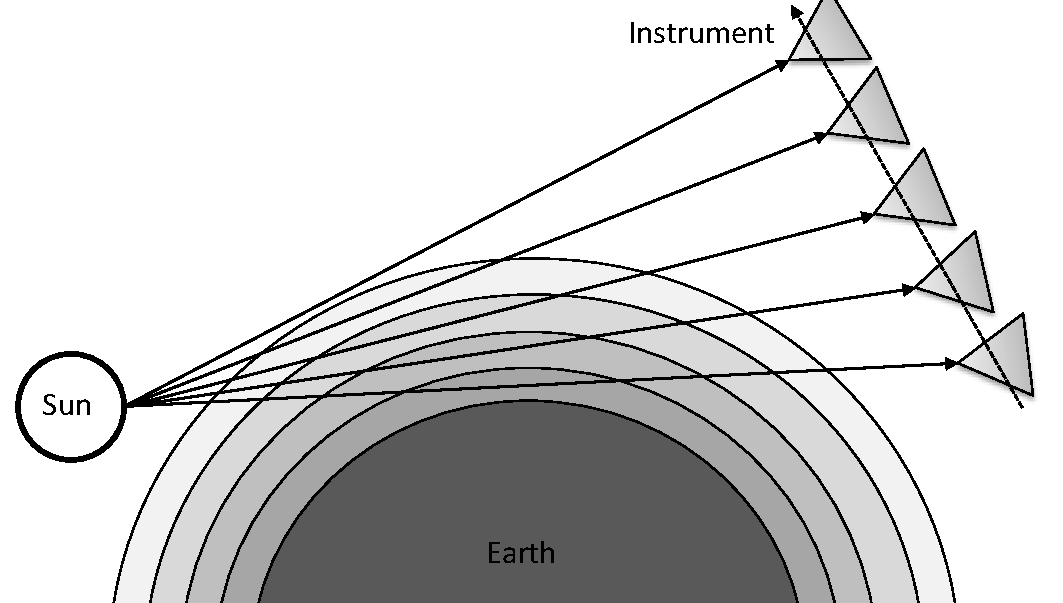
\includegraphics[width=1.0\textwidth]{./Images/OccultationGeometry.pdf}
    \caption[Occultation Geometry]{The occultation instrument monitoring the atmosphere by scanning the atmosphere by looking directly at the sun.}
    \label{fig:OccultationGeometry}
\end{figure}

\subsection{LIDAR}

Through the transmission of a laser pulse though the atmosphere, a method known as LIght Dectection and Ranging (LIDAR) can determine aerosol concentrations through the measuring of the intensity of the backscattered laser light at different wavelengths and polarizations. Initially LIDAR was primarily used at ground based facilities to measure aerosol layers dating back to the 1960s \citep{Fiocco1964}. More recently LIDAR instruments have been used on satellite missions including the Ice, Cloud, and land Elevation Satellite (ICESat) from 2002 to 2010 \citep{Schutz2005} with a second mission, ICESat-2, planed for launch in 2017 and Cloud-Aerosol Lidar and Infrared Pathfinder Satellite Observations (CALIPSO) which launched in 2006 \citep{Winker2007}. Traditional LIDAR instruments have looked in the nadir direction (straight down or up) however some instruments have looked slightly off-nadir, as seen in \autoref{fig:LidarGeometry}, to increases to signal to noise.

\begin{figure}[h]
    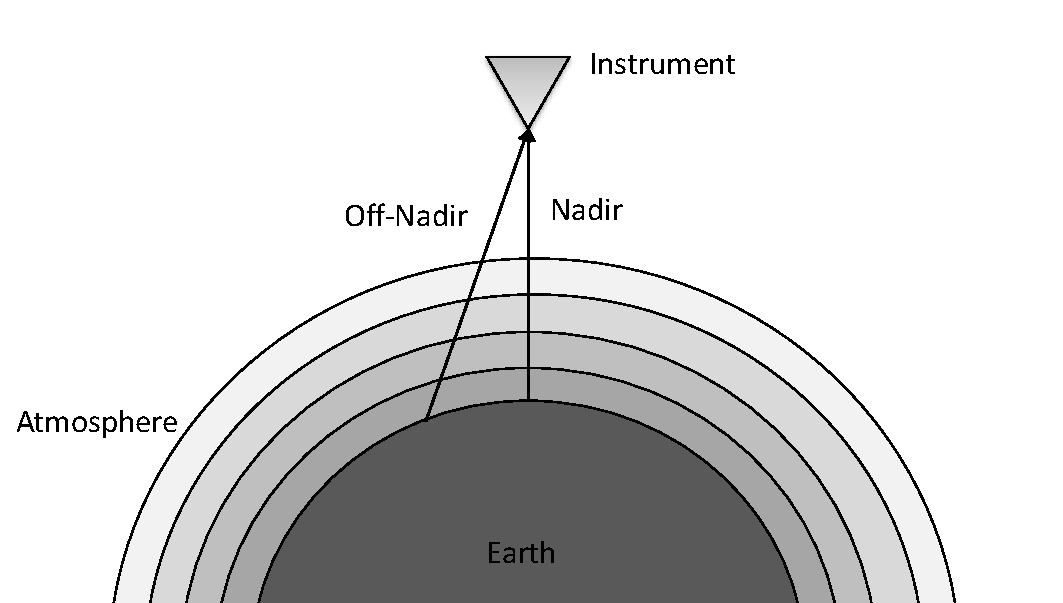
\includegraphics[width=1.0\textwidth]{./Images/LidarGeometry.pdf}
    \caption[LIDAR Geometry]{LIDAR instrument showing a measurement in both the nadir and offnadir lines of sight.}
    \label{fig:LidarGeometry}
\end{figure}

CALIPSO is a joint mission developed between the National Aeronautics and Space Administration (NASA) and the Centre National d'Etudes Spatiales (CNES) of the United States and France respectively. It uses a two wavelength polarized LIDAR system to achieve high resolution aerosol and cloud retrievals along the satellite's orbital track, it views the ground track initially at 0.3\si{\degree} off-nadir to remove specular reflection from still water and then in 2007 the angle was increased to 3\si{\degree} to reduce effects from orientated ice crystals \citep{Hu2009}. CALIPSO data is used to determine aerosol extinction profiles at 40~km horizontal resolution and 120~m vertices resolution with global coverage from 82\si{\degree}S to 82\si{\degree}N \citep{Young2009}. However, despite the excellent vertical resolution given by LIDAR satellite instruments they suffer from poor Signal to Noise Ratio (SNR) especially during the during daylight hours and for high altitude aerosol measurements \citep{Kacenelenbogen2011}.


\subsection{Limb Emission}

MIPAS and MLS (I think) now have sulphate products


\subsection{Limb Scatter}

\begin{figure}[h]
    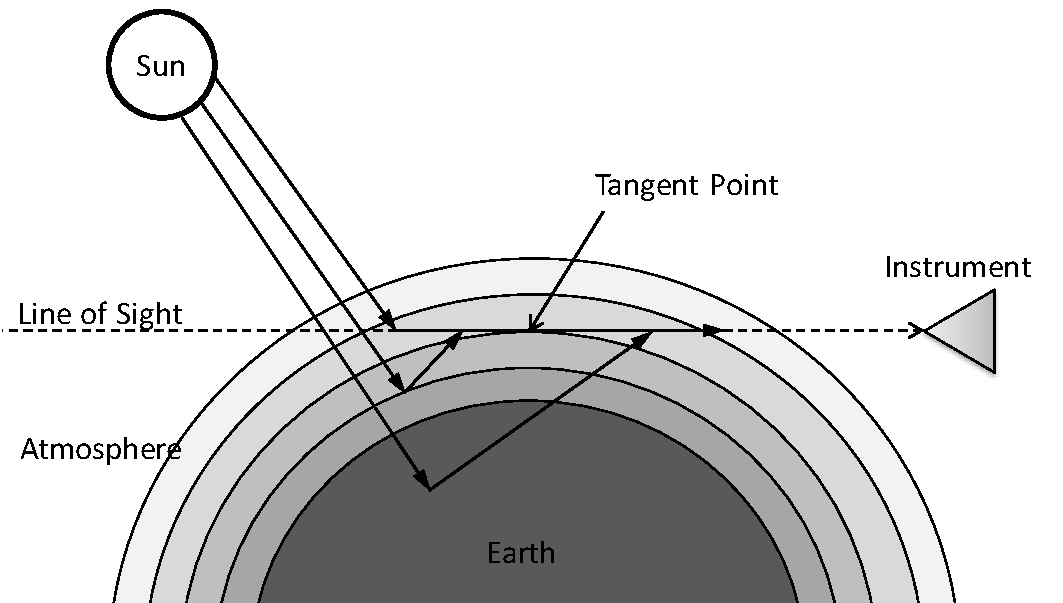
\includegraphics[width=1.0\textwidth]{./Images/LimbScatterGeometry.pdf}
    \caption[Limb Scatter Geometry]{TODO: Write this}
    \label{fig:LimbScatterGeometry}
\end{figure}

\subsubsection{Scanning}

SCIAMACHY OSIRIS

\subsubsection{Imaging}

OMPS and ALTIUS 
\section{The Need for Higher Spatial Resolution}

FROM COMP:

Aerosol number density in the atmosphere is highly variable and difficult to measure due to the unknowns microphysics, which includes particle size distribution and composition. Current satellite capabilities, such as the measurements made by OSIRIS, are limited to approximately 2\.km vertical resolution and sampling every 500\,km along the track.  Much higher spatial resolution is required for current weather and climate model of UTLS processes: desired resolutions are in the range of 200\,m vertically and tens of kilometres horizontally.  Advances in both detector and filtering technologies allow for new instruments to be designed and built with higher resolutions than in previous generations and allow for the capture of two dimensional spacial images. Current limb scatter measurements, like OSIRIS, are preformed using a diffraction grating or a prism which images a spectrum with a single line of sight which is scanned vertically to produce a final product with two dimensions, a spectral and a spacial dimension. However, a filtering device with good imaging characteristics would allow for images to be recorded with two spacial dimensions. The spectral dimension can occur from taking several images in rapid succession at different wavelengths. These measurements will allow for the determination of fine structures in the aerosol extinction profiles and cloud distributions both in the horizontal and vertical direction with required resolution of 4\,km and 0.5\,km respectively \citep{Adams2009}.

Another issue with current instrumentation is limited spectral range. This renders it difficult to determine aerosol particle size. Work done by \cite{Rieger2012} has shown that measurement vectors for limb scatter are only sensitive to different particle size distributions with samples at and beyond 1000\,nm. In order to retrieve any particle size information, measurements will be needed beyond 1000\,nm, where there is some sensitivity to particle size; however, in order to be able to have good sensitivity to aerosol microphysics spectral images recorded at 1200\,nm and beyond are required.

Asian monsoon, resolving high extinction layers, detecting eruption plumes for aviation, etc 
\section{ALI Prototype And CNES Stratospheric Balloon Flight}

ALI Prototype info here    
\chapter{Optical Design and Testing}

\section{AOTF}

Info about AOTF here.

\subsection{Background and Theory}
\subsection{Calibration and Testing} 
\section{Optical Chain Development}

The system needs to be able to preform high resolution images of the atmosphere using the AOTF as the internal filter. It is an ideal device for space applications since it has no movable parts and a fast RF stabilization time; however, the AOTF limits the optical system to only have two functional layouts since the incoming light must enter the device at less than the acceptance angle. This is the maximum angle light can enter the device and still undergo the diffraction interaction. These two layouts are a telecentric and a telescopic system and will discussed in the following two sections. After, a section about the final decision for ALI will under took with rationalization on why the final design was chosen and a comparison to the Belgium instrument ALTIUS.

%The telescope or afocal system causes a wavelength gradient to be formed across the field of view of the image whereas the telecentric design overcomes this problem but has a larger FWHM \citep{Suhre2004} Currently Atmospheric Limb Tracker for the Investigation of the Upcoming Stratosphere (ATLIUS), a Belgium instrument, is being designed with an AOTF in a telecentric layout to remove the spectral gradient \citep{Dekemper2012}. However, the telecentric confocal system has a burring issue that must be corrected before it can be used in atmospheric spectroscopy.

\subsection{Telecentric System Prototype}
\label{sec:3.2:telecentricSystem}

The first system in consideration is a telecentric system. In order to describe the concept behind the telecentric system a basic ray tracing image is shown in \autoref{fig:3.2:rayTracing} where the three paraxial rays are drawn using a simple biconvex lens. %All the rays start from the top of the object and each travel in a certain path. The first ray called the parallel ray travel along the optical axis until it hits the refractive surface then passes through the focal point on the other side of the lens denoted by $f$. The second ray is called the focal ray and it passes through the object (left) side focal point and then travels parallel to the optical axis once it has interacted with the lens. And third the chief ray travels straight thought the center of the lens. These three rays all intersect on the image (right) side and show the location of the formed image.

\begin{figure}[h!]
    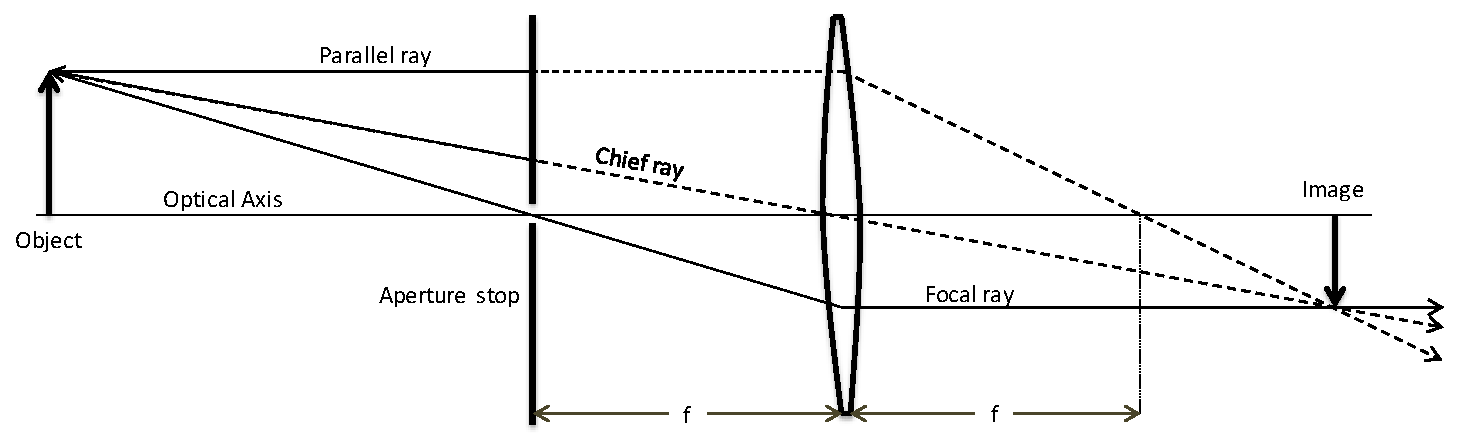
\includegraphics[width=1.0\textwidth]{./Images/3-2-RayTracing.pdf}
    \caption[Telecentric Ray Tracing Diagram]{A standard paraxial ray tracing diagram. The aperture is located to make the system telecentric in the image plane. $f$ is the focal length of the lens.}
    \label{fig:3.2:rayTracing}
\end{figure}

To make this ray tracing system telecentric in image space an aperture is added to the system on the object side at the focal point of the lens. The theoretical idea is to have an aperture so small that only the focal ray can pass through it. All of the other rays, including the chief and parallel ray, are blocked from entering the system. Now the image is only defined by a single ray and it is in focus everywhere on the image side of the system, and therefore has an infinite depth of field. However, a aperture that is so small proposes a few problems in practice. First, a hole of such a small size would cause diffraction effects that would dominate the imaging qualities of the system. Second, such a small aperture would let so little signal through that very long exposure times would be needed or a low signal to noise ratio would result. So in practice a larger aperture is used at the focal point. Now the system no longer has an infinite depth of field, but still retains a large value and the image still remains almost same size no matter where the image plane is located. It should be noted that a telecentric system in object space can be created by putting the aperture on the image side of the lens causing the the object to always be the same size in the image no matter where it is physically located.

%first it would be impossible to make a aperture that is small and is infinitely thin, and

A telecentric layout in both image and object space has an advantage for the imaging quality of the AOTF system shown in \autoref{fig:3.2:telecentricRayTracing}. Since the wavelength filtered by the AOTF is dependant on the incident angle, and from \autoref{fig:3.2:telecentricRayTracing}, all the lines of sight enter with approximately the same angular spread so the filtered image has consistent wavelength. However, two problems are added to the system. First, a blurring effect is added to the final image dependant on wavelength, which will be discussed below in greater detail. As well, this method is sensitive to any surface defects of the crystal since the light enters the crystal in focused bundles.

\begin{figure}[h!]
    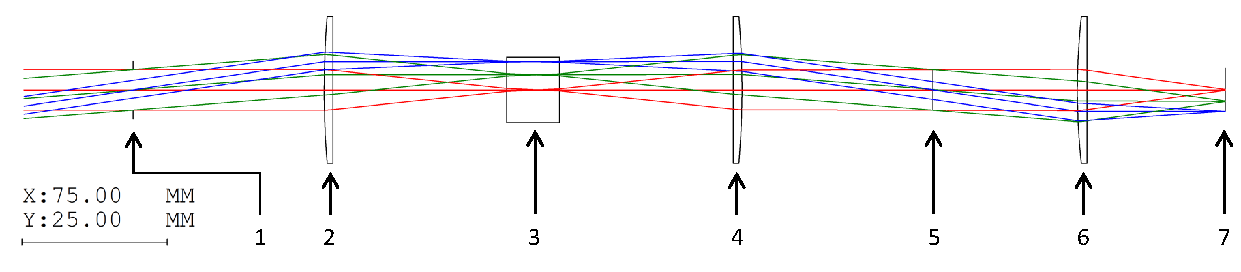
\includegraphics[width=1.0\textwidth]{./Images/3-2-TelecentricRayTracing.pdf}
    \caption[ALI Telecentric Design Prototype]{Ray Tracing diagram simulation of the telecentric lens system preformed using CODE V. The elements in the system are the following: (1) Optical Stop and telecentric aperture. (2) 100~mm focal length plano-convex lens. (3) Brimrose AOTF characterized in \autoref{sec:3.1:AOTFCalibration}. (4) 100~mm focal length plano-convex lens. (5) Telecentric Aperture. (6) 75.6~mm focal length plano-convex lens. (7) Imaging plane. It should be noted that the x and y scales are not the same in this image. Also, in the lab a polarizer is added in front and behind the AOTF as well as prisms after the AOTF.}
    \label{fig:3.2:telecentricRayTracing}
\end{figure}

As a part of this work a test optical system was designed to be telecentric in both object and image space with back end optics to resize the image to fit on the CCD. A list of the specifications can be seen in \autoref{tab:3.2:telecenticSystemParameters} and a ray tracing diagram from a Code V simulation is shown in \autoref{fig:3.2:telecentricRayTracing}. The AOTF has a optical aperture of 10~mm by 10~mm and is the system's field stop. This is a physical limit of the device and causes the field of view to be limited. In order to have lines of sight from the ground to the maximum float altitude of a stratospheric balloon, typically 35~km, a 6\si{\degree} field of view is required. Also with the current set up of 100~mm focal length lenses the rays of light from each line of sight enter the AOTF at the maximum acceptance angle, which is 4\si{\degree}. The acceptance angle is the maximum angle that light can enter the AOTF front aperture and still undergo Bragg diffraction. This allows the maximum amount of light to enter the device and recover the highest throughput as possible.

%However, the aperture of the AOTF limits the system to 5.7 degrees so assuming a 35 km balloon altitude the top kilometer will not be captured by the CCD. In reality this is a negligible loss since the line of sight looking out straight, directly tangential to the earth below, is viewing the least amount of atmosphere compared to any other line of sight, and as such, is not as information dense as lower lines of sight.

\begin{table}[h!]
    \begin{center}
    \begin{tabular}{|l|c|}
    \hline
    Effective focal length (mm) & 75.6 \\
    \hline
    Front optics focal length (mm) & 100 \\
    \hline
    Back optics focal length (mm) & 75.6 \\
    \hline
    Front optics magnification & 1.00 \\
    \hline
    Back optics magnification & 0.756 \\
    \hline
    Field of view ($^{\circ}$) & 5.7 x 5.7 \\
    \hline
    f-number & 14.28 \\
    \hline
    \end{tabular}
    \end{center}
    \caption{Telecentric System Optical Parameters.}
    \label{tab:3.2:telecenticSystemParameters}
\end{table}

The light is focused on a 16-bit digital QSI 616 CCD with a mechanical shutter that allows an integration time between 0.01~seconds to 240~minutes. The CCD chip itself is a Kodak KAF-1603ME with micro lenses to improve the quantum efficiently of the device and its spectral characteristics can be seen in \autoref{fig:3.2:QSIQuantumEfficientcy}.

\begin{figure}[h!]
    \begin{center}
    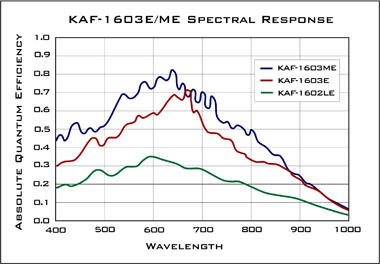
\includegraphics[width=0.5\textwidth]{./Images/3-2-QsiCcdQe.jpg}
    \caption[QSI 616 Camera Quantum Efficiency]{Quantum efficiency of the Kodak KAF-1603ME contained within the QSI CCD camera is represented by blue curve. Quantum efficiency provided by QSI Scientific. }
    \label{fig:3.2:QSIQuantumEfficientcy}
    \end{center}
\end{figure}

The overall design has several aspects that make it a good system for imaging. First all of the bundles of light entering the AOTF have the same angular spread. As seen in equation \autoref{eqn:3.1:AOTFWavelengthDependance} the diffracted wavelength depends on the incoming angle or its spread, in this set up all points of the imaging plane will have the same angular dependance so the entire image will be of the same wavelength and have the same spectral bandpass.

%Also, since the system is telecentric, perspective is not a major factor in the final image of the system as an object of same size but at different distances will appear to be the same size in the recorded image.

However, despite its benefits there are a few drawbacks to consider in the design as well. First, the optical path between the two 100~mm focal length lens is 200~mm in air, however the AOTF is made of TeO$_{2}$  or paratellurite and has a high index of refraction of 2.43 and 2.27 for the extraordinary and ordinary optical axis respectively. The crystal also has a high dispersive property, or Abbe number, so the index of refraction depends on the wavelength. The change is distance in the optical path, $d$, is given by
\begin{equation}
    \ d = \frac{n(\lambda)-1}{n(\lambda)}t
    \label{eqn:3.2:opticalPathDisplacement}
\end{equation}
where $n(\lambda)$ is the index of refraction with a wavelength dependance and $t$ is the thickness of the crystal. The AOTF crystal causes the optical path in air to be lengthened by $d$, as can be seen in \autoref{fig:3.2:opticalPathDisplacement}. In order to compensate, the length $d$ must be added to the path to account to the discrepancy, but this can only be accounted for a specific wavelength and thus image defocusing will occur at the image plane for other wavelengths. The severity of this problem can be seen in \autoref{fig:3.2:telecentricSpotSize} from a Code V simulation of the spot size of the optical system . In this simulation a grid of rays is passed through the system for each field of view and using ray tracing the final locations on the image plane are determined. The black circles represent the Airy disks, which are the minimum possible spot size possible limited by diffraction for each wavelength of light. The above analysis was preformed when the system was focused at 800~nm. The spot sizes at 800~nm are on the order of 24~\si{\micro\meter} at the center, which is diffraction limited, and 94~\si{\micro\meter} at the edge of the field of view. However, for the same optical layout the 600\,nm spot sizes are all greater than 160~\si{\micro\meter} which will cause an noticeable blurring in the recorded image.

\begin{figure}[h!]
    \begin{center}
    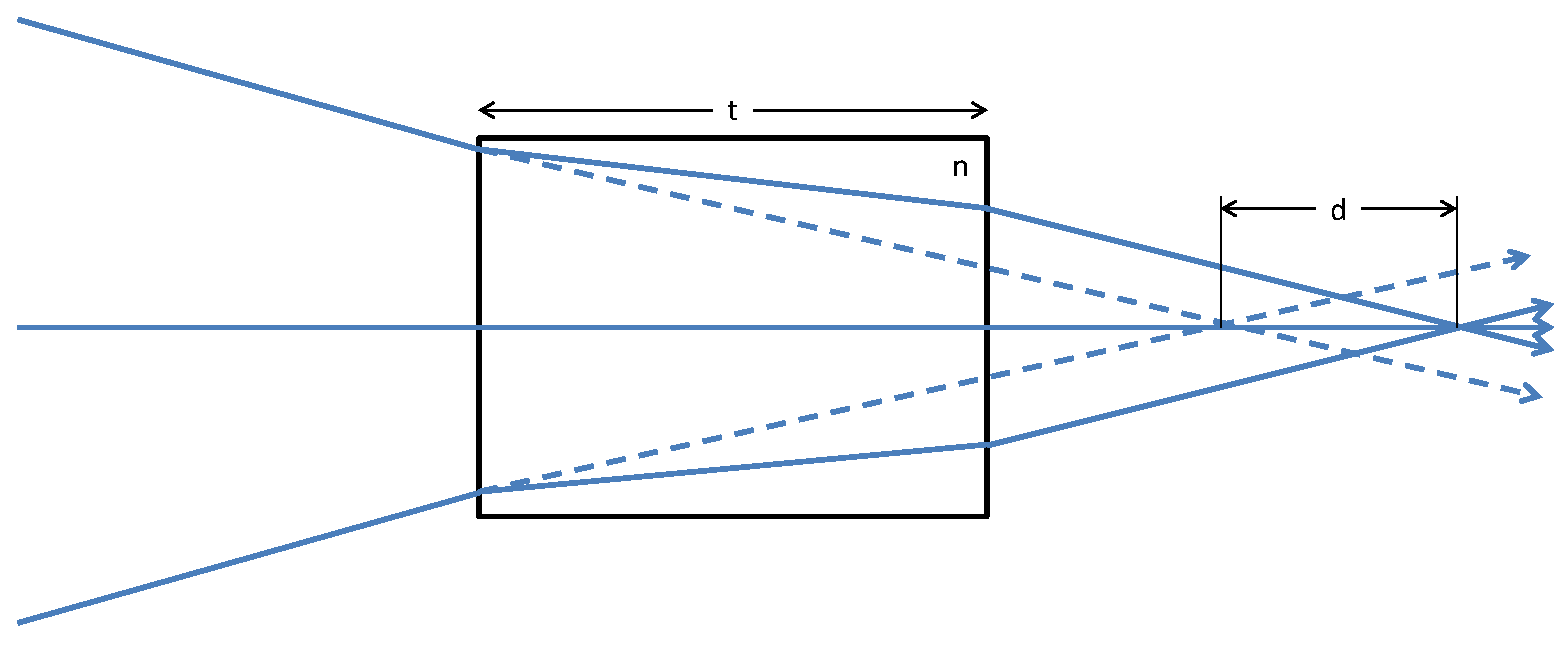
\includegraphics[width=1.0\textwidth]{./Images/3-2-OpticalPathDisplacement.pdf}
    \caption[Telecentric Optical Path Displacement]{TODO: Write Description!}
    \label{fig:3.2:opticalPathDisplacement}
    \end{center}
\end{figure}

\begin{figure}[h!]
    \begin{center}
    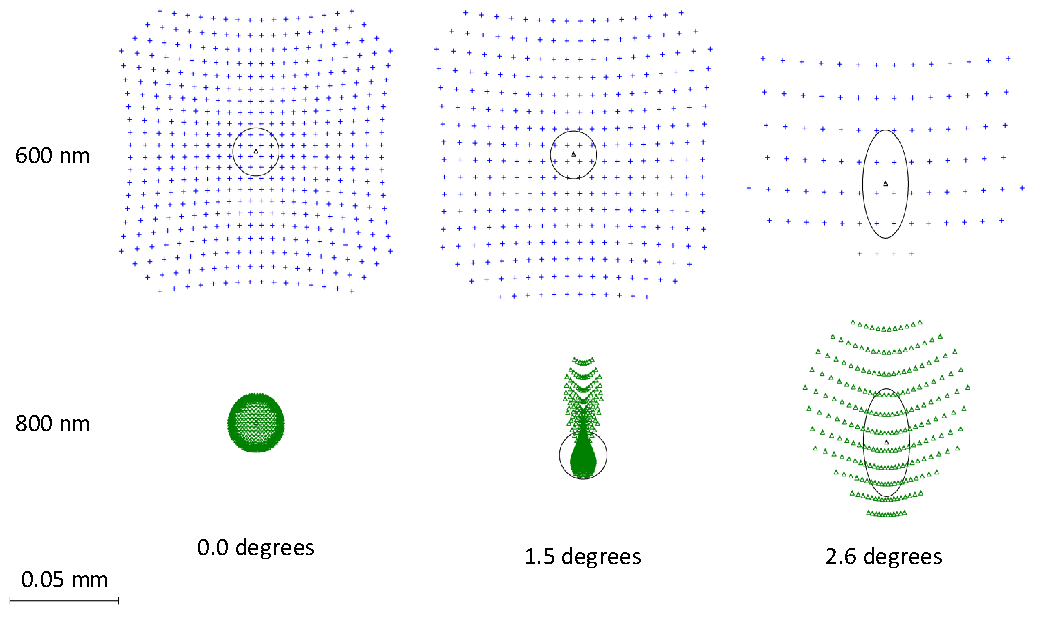
\includegraphics[width=1.0\textwidth]{./Images/3-2-TelecentricSpotSize.pdf}
    \caption[Telecentric Prototype Spot Sizes]{Code V simulation of the spot size for the telecentric system at focus at 800~nm. The spots are shown for 0.0, 1.5 and 2.6 degree fields of view at 600~nm (blue) and 800~nm (green). The full spot sizes for the 600~nm spots are 0.16, 0.22, and 0.25~mm for 0.0, 1.5, and 2.6\si{\degree} fields respectively, with the corresponding 800~nm spot sizes being 0.024, 0.053, 0.094~mm. The black circles represent the Airy disk for each specific wavelength and field of view.}
    \label{fig:3.2:telecentricSpotSize}
    \end{center}
\end{figure}

The system was bread boarded in the lab and used to image EIA 1956 standard resolution chart. The results of the test can be seen in \autoref{fig:3.2:telecentricTestImages}. The experimental set up is similar to the system in \autoref{fig:3.2:telecentricRayTracing} except for two fundamental differences. The Code V software can preform analysis for only one polarization and neglects the bend in the optical axis caused by the AOTF. However, these two issues can be dealt with sufficiently in the lab. The polarization issue is removed by added a polarizer before and after the AOTF. The light that is actively diffracted through the AOTF is the light that enters the AOTF crystal on the extraordinary polarization. The polarizer before the device stops the ordinary polarization from entering the device. The second polarizer on the other side of the device is used to only let the diffracted light through and removes the non-diffracted extraordinary polarization light. The interaction with the crystal causes the diffracted beam to be rotated by 90\si{\degree}, so the polarizers are rotated by 90 degrees with respect to each other. The second issue to be handled is that the AOTF bends the optical path by 2.7\si{\degree}. Two prisms were added after the ATOF to straighten out the optical path; the optical path past the prisms is parallel to the original optical path and is offset by approximately a millimeter and clips a part of the field of the view. The optical layout around the AOTF is similar to the optics around the AOTF in the characterization test shown in \autoref{fig:3.1:testExperimentalSetup}. The resolution chart was positioned so that the loss of the field of the view due to the prism compensation was accounted by a shift in the vertical location of the resolution chart since it only fills the whole field of view in the horizontal direction.

\begin{figure}[h!]
    \begin{center}
    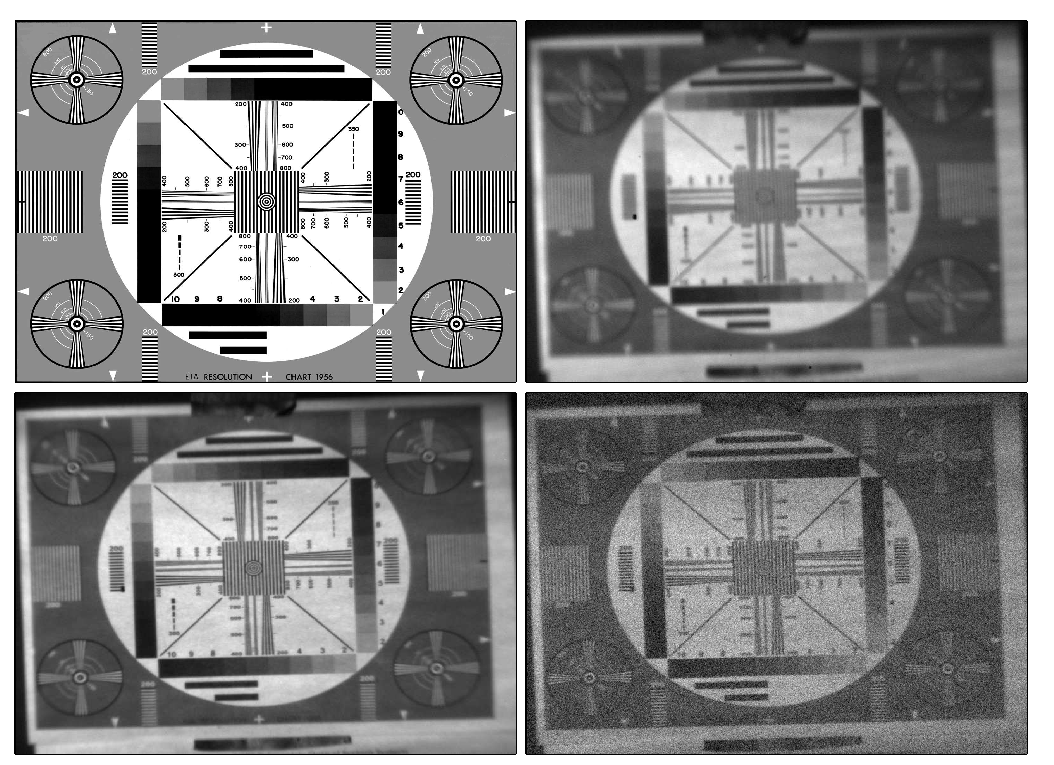
\includegraphics[width=1.0\textwidth]{./Images/3-2-TelecentricTestImages.pdf}
    \caption[Telecentric Prototype Laboratory Test Images]{The top left is the original test image used for the experiment. The top right, bottom left, and bottom right are the images recorded through the telecentric system at 650, 750, and 850~nm. The system is focused at 800~nm.}
    \label{fig:3.2:telecentricTestImages}
    \end{center}
\end{figure}

The images were taken using a 30 second exposures on the QSI CCD for each wavelength with the stray light, dark current, and DC offset removed from the image. From \autoref{fig:3.2:telecentricTestImages} the image blurring that was simulated in the spot size diagram can be easily noticed in the 650~nm wavelength image. The center lines of the resolution chart are unable to be resolved from each other compared to the 750~nm image. A unique line of sight can be resolved every 2 pixels in the center of the 750~nm image which corresponds to 150\,m resolution at the tangent point from the balloon platform, and a 3-4 pixel resolution near the edge corresponding to about a 200~m resolution. Also due to the efficiencies of the CCD the signal to noise ratio at the 850~nm image in the bottom right panel is rather low, and can be visibly seen by looking at the grainy quality of the image and will need to be addressed for the final device. Methods to resolved both of the above issues will be discussed in the future work section.

\subsection{Telescopic System Prototype}

The second optical system in consideration is a telescopic optical system consisting of a standard telescope with a focusing lens at the back end of the optical system. A simple astronomical telescope. The front lens, known as the objective lens, is used to focus an object at infinity to the focal point of the lens, then a second lens, the eyepiece is used to increase the optical power of the system, that is to increase the angular size of the image with respect to the angular size of the object. The eyepiece lens is located at a combined distance of the of the focal lengths of both the objective and eyepiece and causes the image to be focused at infinity. However for our system the telescope is used to focus the light in order to enter the AOTF at an angle less than its acceptance angle as well as to reject light rays outside of our field of view. The light from each line of sight in the telescopic system enters the AOTF collimated and is focused though a focusing lens onto the the QSI CCD discussed in section \autoref{sec:3.2:telecentricSystem}. A detailed simulated Code V layout of the optical design can be seen in \autoref{fig:3.2:telescopicRayTracing}.

%The magnification is given by

%\begin{equation}
%    \ M_{\theta} = -\frac{f_{o}}{f_{e}}
%    \label{eqn:telescopeMagnification}
%\end{equation}

%where $M_{\theta}$ is the optical power or the angular magnification, and $f_{o}$ and $f_{e}$ are the focal lengths of the objective and eyepiece respectively.

\begin{figure}[h!]
    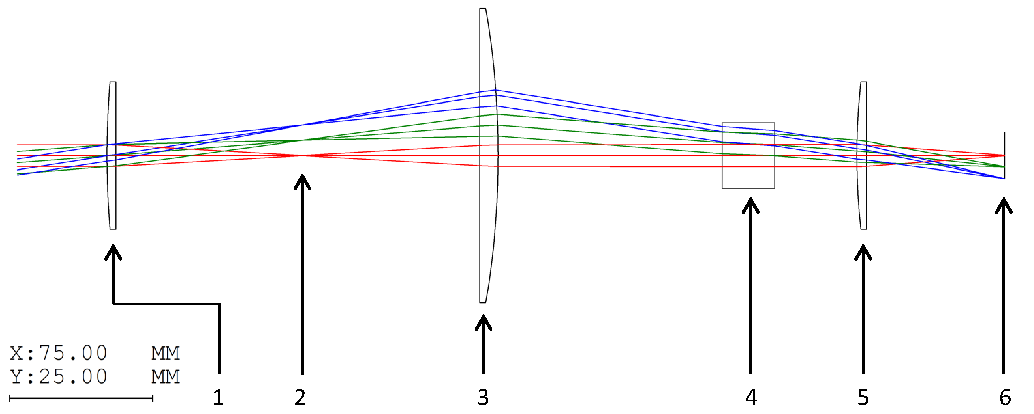
\includegraphics[width=1.0\textwidth]{./Images/3-2-TelescopicRayTracing.pdf}
    \caption[ALI Telescopic Design Prototype]{Ray Tracing diagram of the telescopic lens system simulated by Code V. The elements in the system are the following: (1) 100~mm focal length plano-convex lens. (2) Location where shutter will be located to limit stray light (3) 100~mm focal length plano-convex lens. (4) Brimrose AOTF characterized in \autoref{sec:3.1:AOTFCalibration}. (5) 75.6~mm focal length plano-convex lens. (6) Imaging plane. It should be noted that the x and y scales are not the same in this image. Also, in the lab a polarizer is added in front and behind the AOTF as well as prisms behind the AOTF.}
    \label{fig:3.2:telescopicRayTracing}
\end{figure}

This system was designed with as many similar components as possible to the telecentric system in order to allow comparisons of the system to be made without major optical effects and abberations caused by using different materials, sizes, and focal length lens. The optical specifications of this system are given in \autoref{tab:3.2:telescopicSystemParameters}. However, there are fundamental differences, the aperture stop is located at the front lens which limits the rays of light that can enter the system, unlike the telecentric design that has a front aperture at the focal length of the first lens.

%Therefore, this system has perspective in the final image, meaning objects further away look smaller in the final image.

\begin{table}[h!]
    \begin{center}
    \begin{tabular}{|l|c|}
    \hline
    Effective focal length (mm) & 75.6 \\
    \hline
    Front optics focal length (mm) & 100 \\
    \hline
    Back optics focal length (mm) & 75.6 \\
    \hline
    Front optics magnification & 1.00 \\
    \hline
    Back optics magnification & 0.756 \\
    \hline
    Field of view ($^{\circ}$) & 6.0 x 6.0 \\
    \hline
    f-number & 20 \\
    \hline
    \end{tabular}
    \end{center}
    \caption{Telecentric System Optical Parameters.}
    \label{tab:3.2:telescopicSystemParameters}
\end{table}

The AOTF now has collimated light passing though the device, unlike the telecentric system, and this has a few fundamental changes to alter to the system's imaging quality. First, the primary light passing through the AOTF from a single line of sight is entering the AOTF at the same angle, so the image will have a smaller FWHM than the telecentric counterpart however each line of sight will be diffracted with a different fundamental wavelength due to the angular dependance in the AOTF Bragg diffraction wavelength determination equation (\autoref{eqn:3.1:AOTFWavelengthDependance}). The final image has a smaller spectral bandpass but there will a wavelength gradient radiating out from the center of the image. Second, since the light now passes through the AOTF collimated, the focal point of the image no longer changes with wavelength. Instead a lateral displacement of each line of sight occurs based on the angle of incidence and the diffracted wavelength which causes a slight magnification of the image. The lateral displacement that occurs is given by the following relation
\begin{equation}
    \ \delta = (n(\lambda)-1)\frac{t\theta}{n(\lambda)}
    \label{eqn:3.2:planeParallelDiplacement}
\end{equation}
where $\delta$ is the displacement from the original path; causing a slight magnification change based on the wavelength of the light being diffracted, but this magnification is a negligible change overall, the effect can be seen in \autoref{fig:3.2:planeParallelDiplacement}. The last change to the system is the focusing power it possesses, as can be seen in the spot diagrams in \autoref{fig:3.2:telescopicSpotSize}. The change in spot size due to wavelength is primarily due to the chromatic aberrations of the optical lens. One option is to replace the lenses with mirrors in the flight version which will eliminate the chromatic abberation issue. Second, the system is diffraction limited for 600\,nm for all lines of sight and at 800\,nm at 3.0 degrees. Also the difference in location of the spot sizes is caused by the magnification effect discussed above.

\begin{figure}[h!]
    \begin{center}
    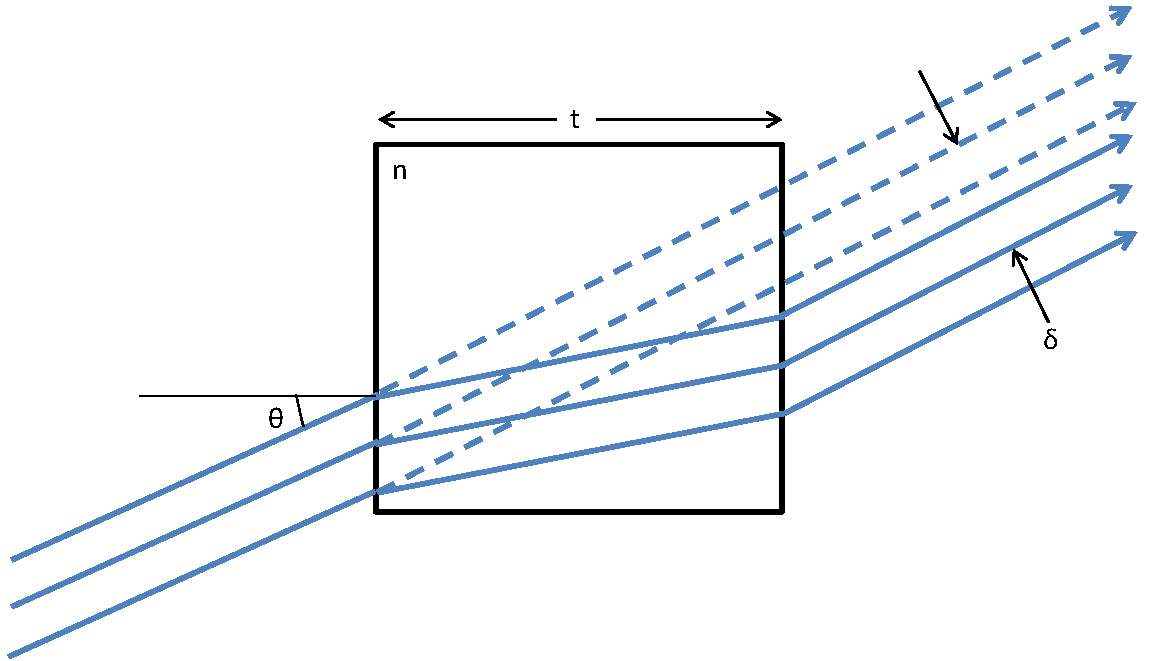
\includegraphics[width=1.0\textwidth]{./Images/3-2-PlaneParallelDisplacement.pdf}
    \caption[Telescoptic Plane Parallel Displacement]{TODO: Write Description!}
    \label{fig:3.2:planeParallelDiplacement}
    \end{center}
\end{figure}

\begin{figure}[!h]
    \begin{center}
    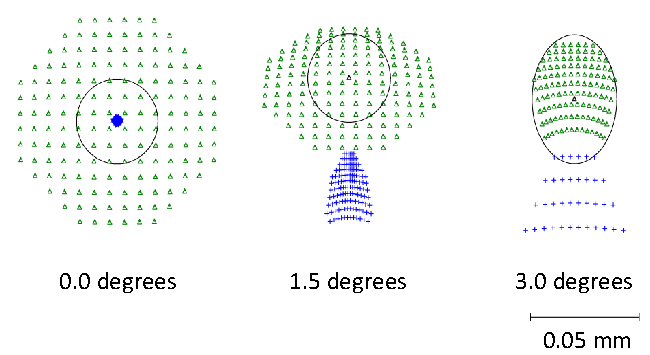
\includegraphics[width=0.70\textwidth]{./Images/3-2-TelescopicSpotSize.pdf}
    \caption[Telescopic Prototype Spot Sizes]{Code V simulation of the spot size for the telescopic system. The spots are shown for 0.0, 1.5 and 3.0\si{\degree} fields of view at 600~nm (blue) and 800~nm (green). The full spot sizes for the 600~nm spots are 0.004, 0.045, and 0.122~mm for 0.0, 1.5, and 3.0\si{\degree} fields respectively, with the corresponding 800~nm spot sizes being 0.096, 0.081, 0.047~mm. The black circles represent the Airy disk for each specific wavelength and field of view.}
    \label{fig:3.2:telescopicSpotSize}
    \end{center}
\end{figure}

An experimental resolution test was set up similar to the one described in \autoref{tab:3.2:telecenticSystemParameters} with two polarizers and prisms added to the optical chain. The QSI CCD was also used with the same 30 second integration time. The results of this test can be seen in \autoref{fig:3.2:telescopicTestImages}. Once again the image at 750~nm is the sharpest of the three but the center lines of the EIA 1956 test chart are distinguishable at all of the wavelengths. The blurring of the 650~nm image is caused by the chromatic abberations of the lens and the prisms and will removed if mirrors are used in the final design. Also, the magnification issue discussed above is relatively insignificant in the test images and the small changes can be accounted for in the calibration of the final instrument. Lastly, the low NIR levels of the light source combined with the poor quantum efficiency of the CCD camera causes the 850~nm image to also have a low signal to noise ratio. This issue will have to be dealt with in the final design, which as mentioned may include an InGaAs sensor array. A final note to be made is the gradient found in the brightness of these images. This is currently thought to be a vignetting problem due to an optical misalignment and is under investigation.

\begin{figure}[h!]
    \begin{center}
    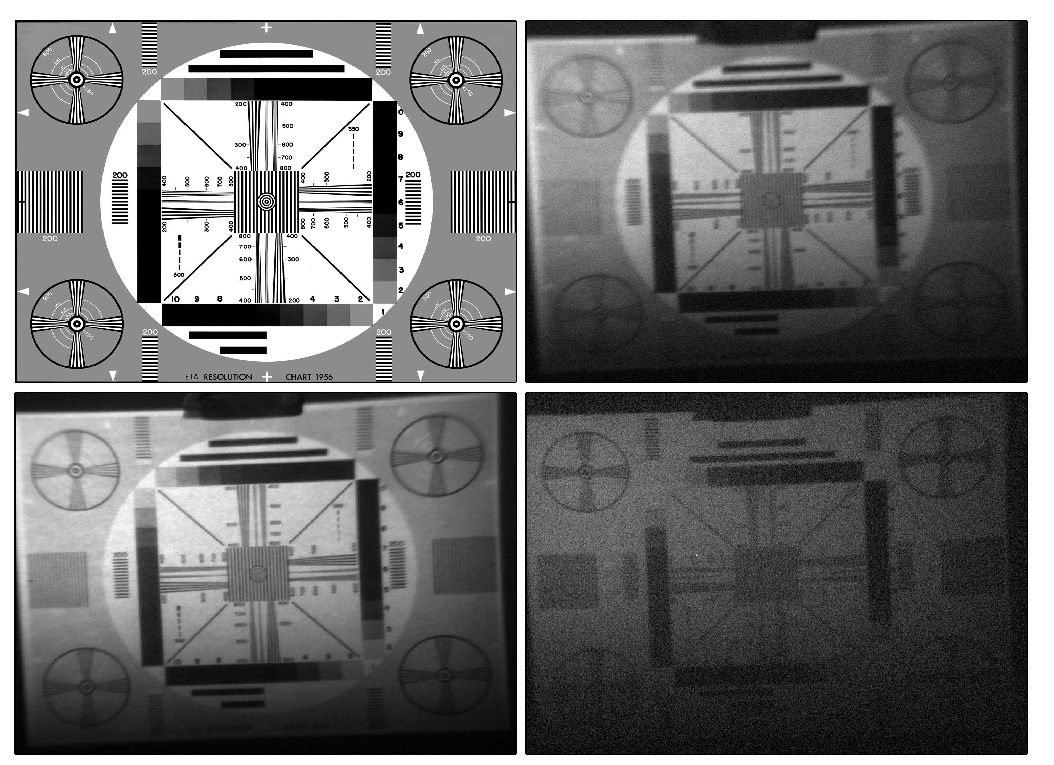
\includegraphics[width=1.0\textwidth]{./Images/3-2-TelescopicTestImages.pdf}
    \caption[Telescoptic Prototype Laboratory Test Images]{The top left is the original test image used for the experiment. The top right, bottom left, and bottom right are the images recorded through the telescopic system at 650, 750, and 850\,nm. The system is focused at 800\,nm.}
   \label{fig:3.2:telescopicTestImages}
    \end{center}
\end{figure}

\subsection{Final Choice}

A final selection for the optical design of ALI will be presented in this section as well the justifications used to determine the result. Furthermore, a comparison with the prototype Belgium instrument will be made to demonstrate the differences between the two instruments. For the final design of ALI the telescopic system deemed to be the better option for our scientific purpose to determine aerosol extinction and engineering study to verify the capabilities of using an AOTF in space based remote sensing techniques.

The telescopic system offers the ability of having an image plane location that is not dependant of the wavelength being imaged leading to a system that would either require the system to have mechanical pieces to move the imaging plane or additional optical components to counter act the change in the optical path. Using mechanic components to move the camera would be an addition failure point and would have to be well calibrated across the whole wavelength range. Adding addition

discuss similarities and differences with ALTIUS specs from Dekemper et al paper



From progress Report:

he next critical step for the ALI instrument was to decide between the two designs, a telecentric and a telescope system, for the optical chain. After some investigation of the advantages and disadvantages between each system the telescopic system was chosen for the final optical design for ALI. This system allows the image plane of the system to be at consistent position for all wavelengths that are measured; therefore fewer mechanical and optical components are required to counterbalance the change in the location of the image plane that is seen in the telecentric system. Thus leading to an increase in throughput by not adding correcting optical components and a reduction of the chance of a mechanic failure during flight. The two primary issues with the telescopic system, the wavelength gradient and the wavelength dependant magnification, can both be removed from of the final data product with calibration measurements preformed before the launch.

Once the optical design had been finalized, the bread boarded optical system was redesigned into a flight version and built. First, the optical specifications were chosen based on light throughput required for 2-3~second exposure times on the balloon, as well to be a reasonable size to be able to fit on the balloon platform. Unfortunately, due to the launch of the balloon being a year earlier than originally estimated the idea of building a folded optical system for ALI is no longer possible due to time constraints. The specifications of the optical system can be seen in \autoref{tab:3.2:ALISystemParameters}. Front end magnification is preformed in order to increase the throughput of the system with the constraint of the  the active optical aperture of the AOTF. The final image size is 1000x1000 pixel with each pixel having a size of 9~$\mu m$. ALTIUS, a Belgium instrument, uses similar technology as ALI except uses a telecentric optical layout and is designed to measure atmospheric trace gasses \citep{Dekemper2012}. The optical specifications are similar between the two instruments, however two differences will be noted. First, the field of view of ALTIUS is smaller at 5.73x5.73\si{\degree} and if ALI was to have used a telecentric design then it would have had an identical field of view. In a telecentric design the AOTF aperture directly limits your instruments field of view and both system use an ATOF crystal with an optical aperture of 10x10~mm. Second, the f-number for ALTIUS is 14.32 compared to ALI's 7.5 which allows ALI to increase light throughput at the cost of higher abberations in the final image.

\begin{table}[!ht]
    \begin{center}
    \begin{tabular}{|l|c|}
      \hline
      Effective focal length (mm) & 74.3 \\
      \hline
      Front optics magnification & 0.67 \\
      \hline
      Back optics magnification & 1.27 \\
      \hline
      Field of view (\si{\degree}) & 6.0 x 6.0 \\
      \hline
      F-number & 7.5 \\
      \hline
      Image Size (mm) & 9x9\\
      \hline
      Spectral Range (nm) & 650-950\\
      \hline
    \end{tabular}
    \end{center}
    \caption{ALI Final System Optical Parameters.}
    \label{tab:3.2:ALISystemParameters}
\end{table}

\subsection{Calibration and Testing}

\section{BaffleDesign}

A BASIC START:

Many questions arose when the baffle for the ALI system was devised. Questions arose over length and width of the baffle as well as how many baffles should located in the final design as well as the interior shape of the baffle layout. These were all important questions that needed ansering since stray light rejection from the ALI insturment is crutial in order to achieve high sensitivity of the light from the atmoshere.

The baffel system is designed such that all light entering the system hit at least 3 surfaces before it can enter the opical system for direct scattering and 2 surfaces for indirect scattering. This methoid is called the thriple bounce disign and i standeredly used in opticals to minimise stray light. In the system the baffels are spaced in such that no stray light that can enter the system is minimized by having the stray light hit three incoming surfaces reducing the overall intersity of the light.

The first point of the discussion was a hight versus width discussion. IN a baffle system the larger the baffle is by shear volume the better the baffle can be designed to reduce stray light. However there is a limited amount of space to build the ALI instrument and the baffle must share space with optics, eletronics and power systems; as such a size had to be selected. A height and width of 70 mm was choosen. The CCD camera used in the design had a height of a little greater then 70 mm and did not want the instrument to have to be any taller. This left the length of the baffle to be determined. The length is also limited by the space for ALI as well as the field of view and entrance apperture size, and its location. One always needs to make sure the the optical stop is the location that limits the amount of light that is entering the system. If this is artifically changed with the baffle design it will affect the preformance of the instrument itself. If the optical stop is moves further from the optical system one keeps the same field of view but limits the amount of light that enters the system. Thus changing the overall F/\# of the system and either increases the exposure times or decreases the signal to noise ratio. The other case is if the optical stop is moved closer to the optical system, which causes the opposite problem which is more light enters the system than the system was designed for causing an excess of stray light and rendering the baffel useless.

This information leaves us with three kinds of fundimental locations to put the optical stop of the system in the design phase. The first is to put the optical stop as close ot the front lens as possible, second is to place the optical stop at the far end of the baffel, and third to place the optical stop in the middle of the baffle system. IN the first case the baffels have a  diverging shape and there are few baffles. In the second case

Although the overall choice between these three do not have  a great effect on the effencey of the baffle itself it has an effect on the shape on the baffle system as well as the number of baffles required. The greatest difference is the change in the optical system required, the further away the optical stop is from the front lens the larger the optical components need to be in order to accept all of the light, which makes the system heavier, larger and more expensive to build. In ALI the optical the stop was choosen to be close to the first lens to make the system has small and compact as possible as well has to reduce the number of baffels that needed to be built for the system and thus the overall cost with reducing the systems effectivness.
 
\chapter{Polarization Study} 

Info and Sections to be added later. General current Idea below

    4.1 SASKTRAN radiative transfer model
        4.1.1 Background
        4.1.2 Hi-Res Model
        4.1.3 Monte Carlo Model
    4.2 Effect of polarization on radiance from satellite geometry in an aerosol atmosphere
    4.3 Effect on aerosol retrievals (sensitivity as a function of wavelength and scattering/zenith angles)

\chapter{Stratospheric Balloon Flight and Data Analysis} 

Gernal Info goes here

\section{Preparations and Flight Day}

The balloon launch base in Timmins, Ontario is located at 48.47\si{\degree}N 81.33\si{\degree}W and ALI arrived at the base located at the Victor M. Power Airport on August 25, 2014 with a launch window from September 8 to 14, 2014. In between the arrival and launch ALI had to be verified to have survived transportation, a seal within the CCD needed to be removed, thermal insulation was to be added, and finally ALI needed to be integrated onto the CNES CARMEN-2 gondola. ALI was unpacked at set up on a test bench at the launch facility and a visual inspection occurred to verify that no obvious damage occurred to the instrument during transportation. Once completed, ALI was connected to its electronics and and power boxes and power was enabled to the ALI and a local computer was used to connect to the device and verify that the system powered on correctly and that the science operation program was activated during startup. At this point it was verified that no functional problems occurred to the device during transportation, all temperature and voltage sensors, GPS module, and CCD camera were reporting diagnostic values as expected. Once the ALI system was verified to be operational an imaging check was performed to check on the optical components survived the trip. A EIA 1956 resolution target was illuminated by a 250~W tungsten halogen light source and was imaged by ALI to verify the optical layout. The recorded images were very similar to the one taken in the laboratory before the leaving Saskatoon.

Following the successful test of ALI a few final preparations were needed prior to beginning integration with CARMEN-2. First, The instrument CCD had a sealed chamber that was in a vacuum state designed to be at one atmosphere of pressure and would be required to be unsealed before the flight. The unsealing is done in order to not develop a strong pressure gradient between the CCD chamber and the low pressure 35~km environment causing permanent damage to the CCD detector itself. At the launch facility ALI was taken to a semi-clean area to unseal the CCD chamber. A panel was removed on the side of the camera and the seal to be removed can be seen in \autoref{fig:5.1:ccdVacuumUnsealing}. The orange o-ring was removed with associated sealing components and the vacuum seal was broken. The chamber panel was replaced and ALI was move back to the integration hall and another set of test resolution targets were taken to verify the correct operation of the ALI. All resolution target looked similar with from the set before the chamber was unsealed expect there was approximately a 5\% drop in counts which was excepted of the device.

\begin{figure}
    \center
    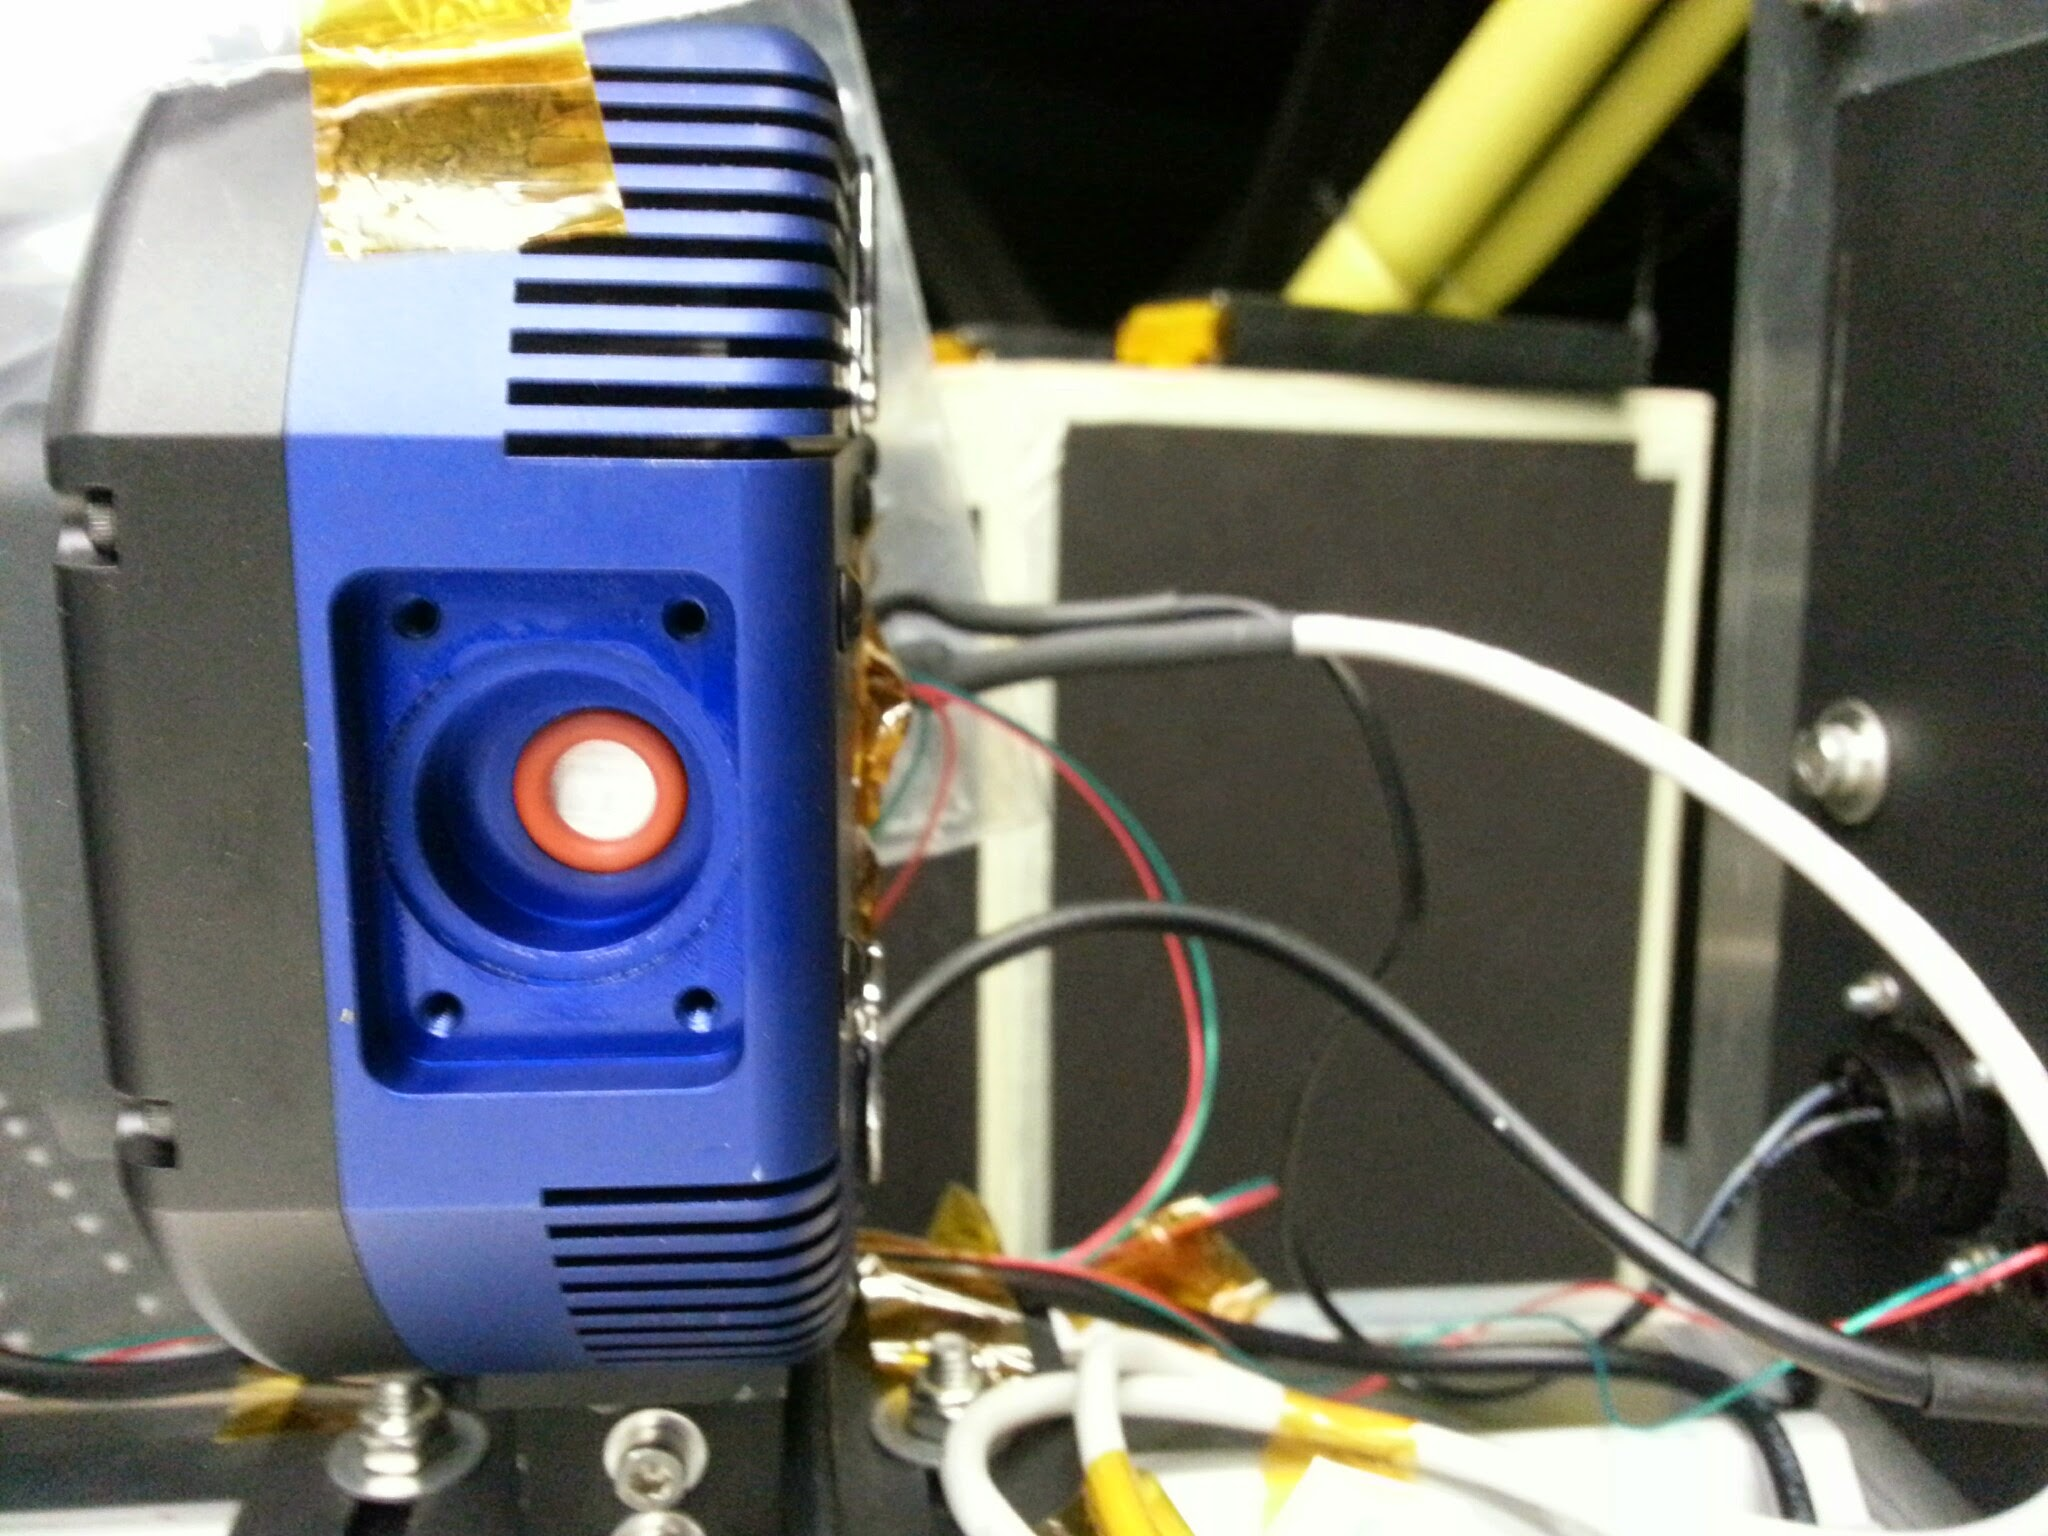
\includegraphics[trim={0 150 1200 0},clip,width=0.5\textwidth]{./Images/5-1-CCDVacuumUnsealing.jpg}
    \caption[QSI CCD Vacuum Sealing O-ring]{Side of the QSI CCD with the panel that contains the vacuum seal opened. The orange o-ring removed seen in the cavity is removed from the chamber to open the vacuum seal to the camera's CCD chip.}
    \label{fig:5.1:ccdVacuumUnsealing}
\end{figure}

 After the competition of the verification of the ALI system, work was done in order to protect ALI from the thermal environment at approximately 35~km. The first concern was the instrument reaching a temperature that was too cold to function. The instrument would have to spend some time during the initial rise in complete darkness which would result in little to no solar heating as well as pass through the tropopause where temperature can be as cold as -70\si{\degree C}. Insulation, in the form of Styrofoam, was added around the exterior of the instrument to help give ALI some thermal isolation from the environment. A second concern was once CARMEN-2 was at float altitude ALI would have to be able to survive the direct heating from the sun's radiation. The impact of the sun's energy was reduced on ALI by adding a thermal reflector to the outside of the thermal insulation expect to come into contact with the sun's radiation to reduce effects from direct heating which could cause overheating in either the optical chain or electronics boxes. The reflectance material was supplied by the CNES CARMEN-2 team and the full system with thermal management component can be seen in \autoref{fig:5.1:aliIntigratedOnCarmen}.

 \begin{figure}
    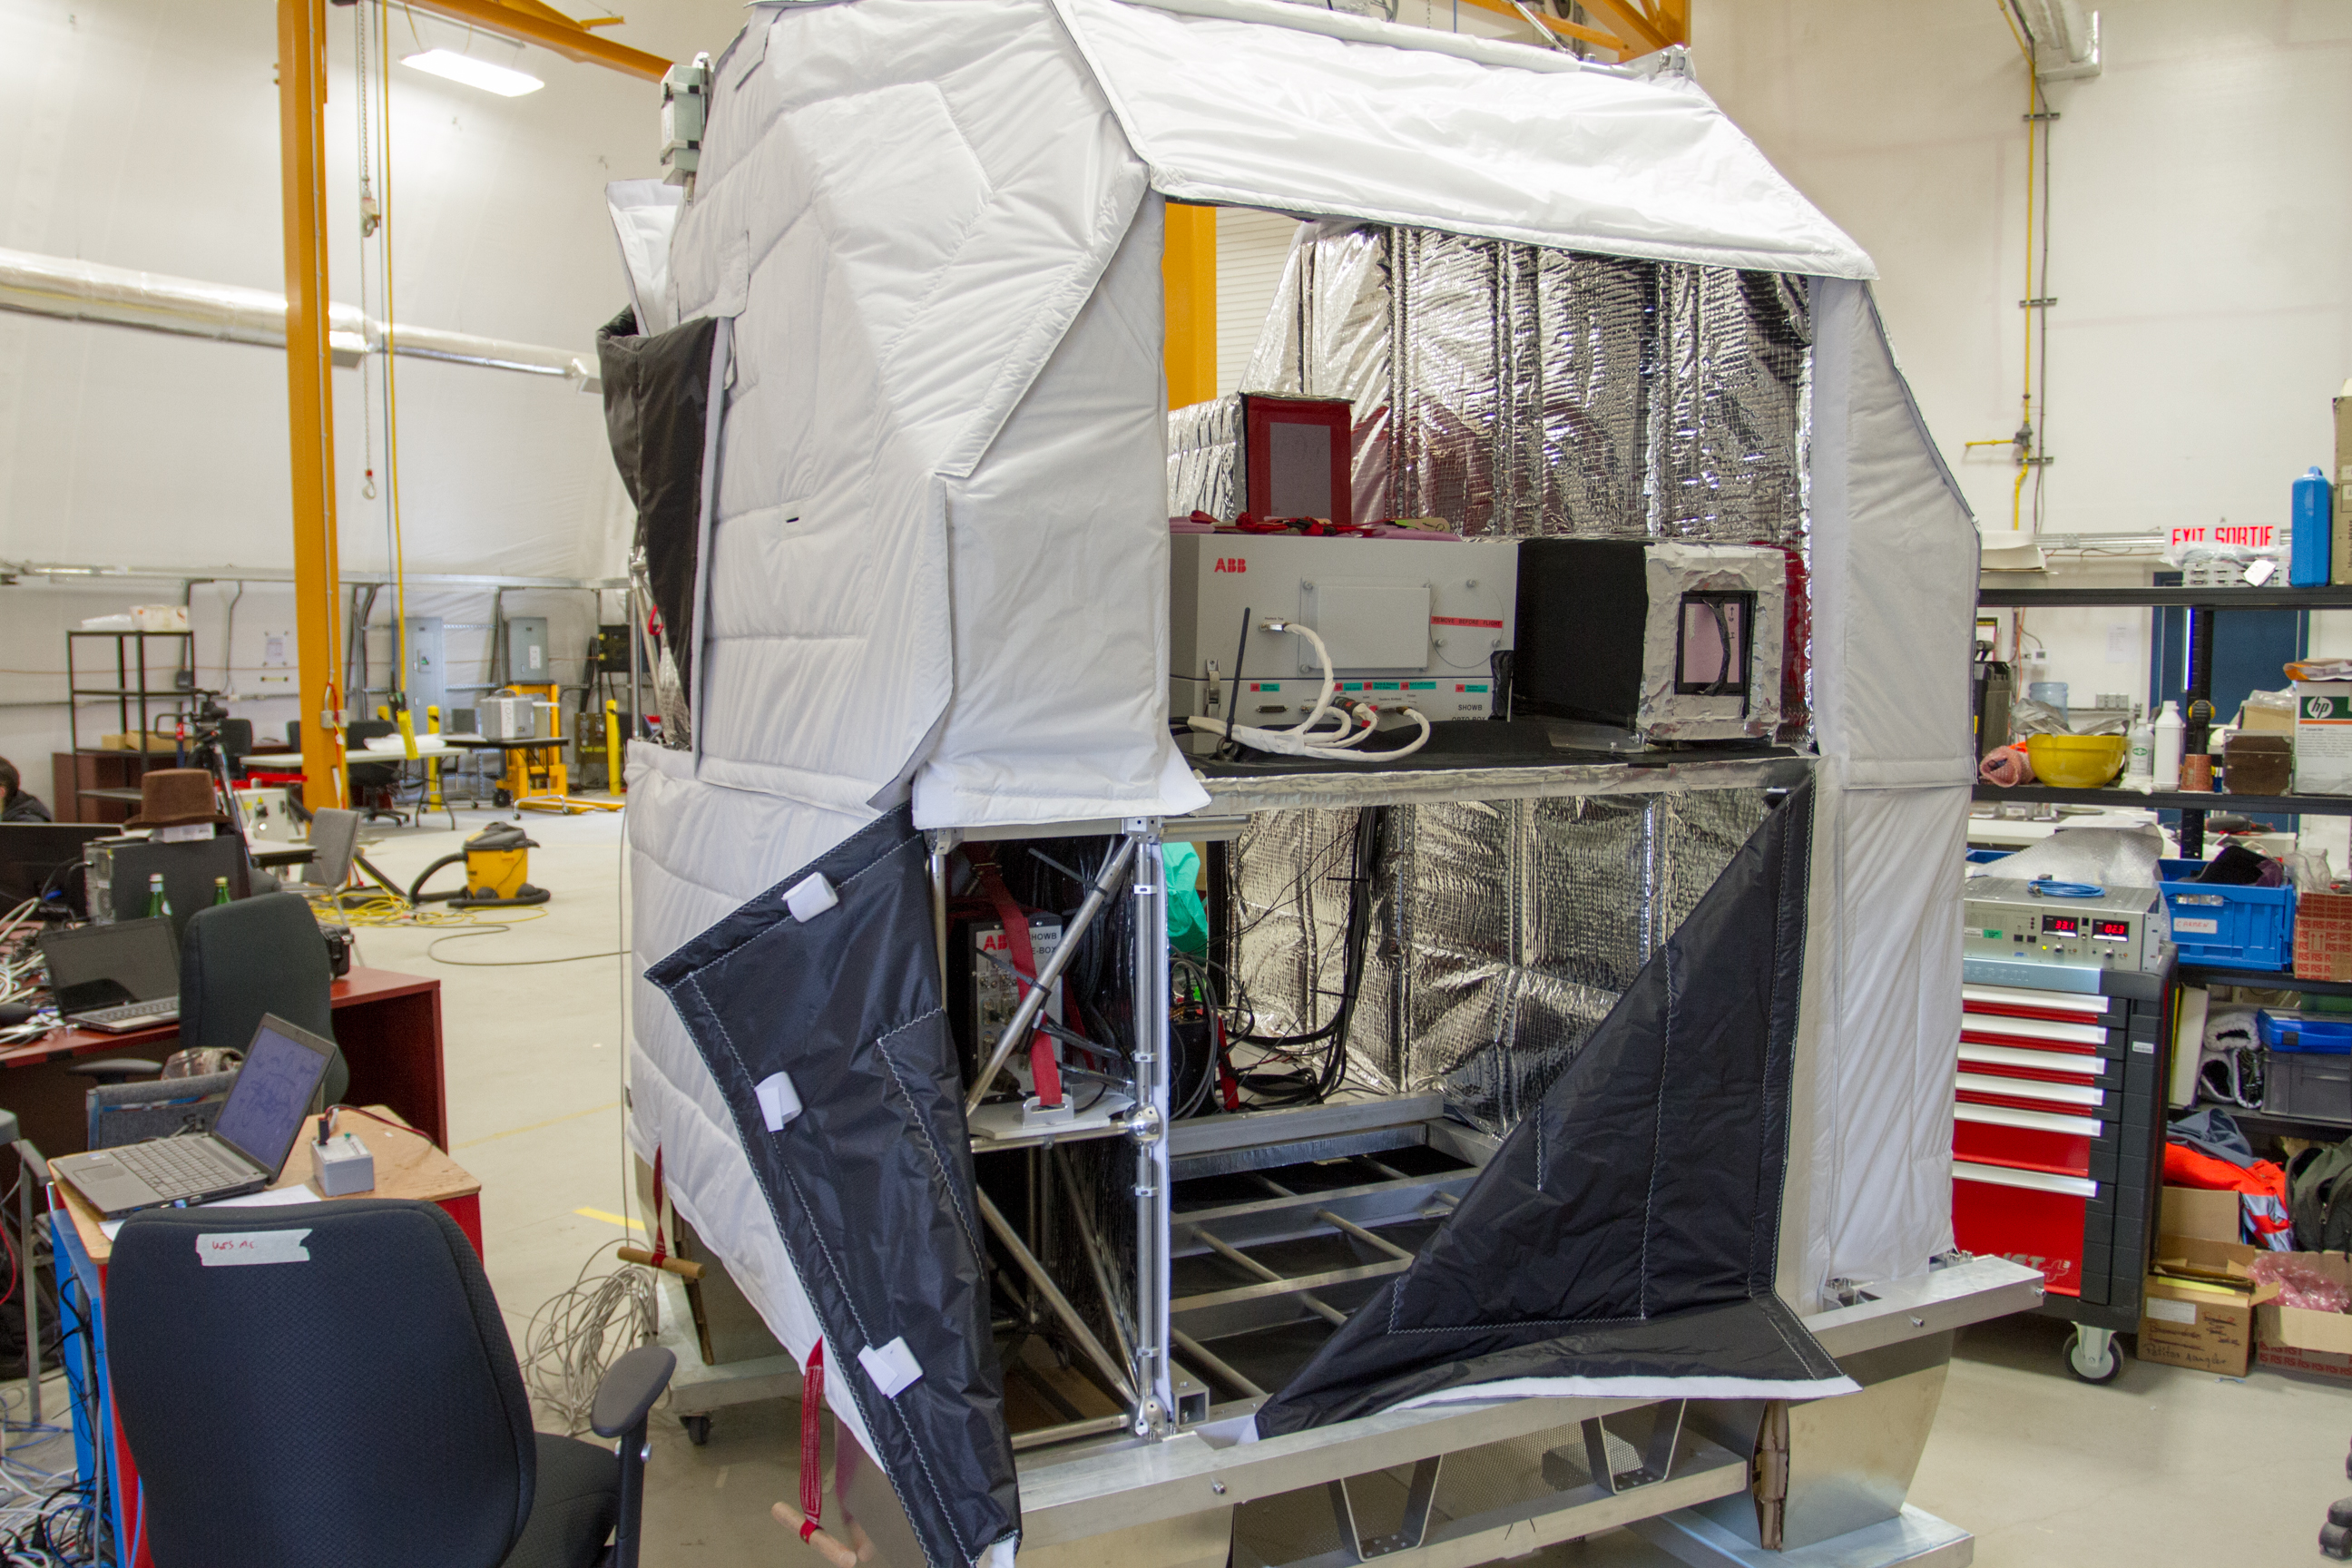
\includegraphics[trim={900 800 500 0},clip,width=0.7\textwidth]{./Images/5-1-AliIntegratedOnCarmen.jpg}
    \caption[ALI Mounted onto the CARMEN-2 Gondola]{The ALI instrument is mounted on board the CARMEN-2 gondola located next to SHOW, another Canadian instrument with collaboration between ABB, York University, and the University of Saskatchewan. Ali has its red tag cover over the optical entrance to protect the instrument from dust and other contaminates. Thermal insulation has been added to the instrument and during the flight sun side will be on the side of SHOW. Some of the reflective layer was blacked out to not cause additional stray light into SHOW optical path. With this geometry ALI will be pointed primarily to the south during the mission at approximately 90\si{\degree} from the sun.}
    \label{fig:5.1:aliIntigratedOnCarmen}
\end{figure}

After the completion of the thermal management, work was done to verify that ALI worked with the CARMEN-2 control systems and to be mounted to the gondola. Connections were verified for power and communication lines to integrate onto the CARMEN-2 system. Power lines operated as expected with no problems and there was no issues with the internal communication. However, when connection with ALI was attempted between the ground station no connection could be established. The external communication system known as the Siren module used a different ethernet setup that was used in the lab to establish a connection. Modifications were made to the flight and ground software to account for the Siren requirement and the system was retested, this time with full connection and little for UPD data losses, of which some are expected due to the nature of UDP communication. After verification ALI was mounted, with the help of the CARMEN-2 team, onto the gondola in preparation of the balloon flight. During this integration phase it should be noted that several instruments were also being verified with the CARMEN-2 systems for integrated onto the gondola including four other Canadian instruments, including a modification to the OSRIS Development model, and SHOW to measure water vapour.

The CARMEN-2 gondola itself is a pointed gondola that is piloted from the ground station in Timmins, in the case of communication failure occurs the balloon can also be piloted by a backup team located in France. The general pointing of the system is done by the CARMEN-2 control systems and once control is established a French star tracker, ESTADIOS, is used in order to further fine tune the pointing of the gondola with better to 1\si{\degree} accuracy.

The flight plan for the CARMEN-2 gondola was to have a near sunrise launch and once altitude was reached ALI, OSIRIS, and SHOW would preform their operational missions for the first four hours of the campaign followed by a scan in the azimuth direction for instrument sensitivity for ALI. During this time ALI would preform several primary mission operations including a dark imaging suite for calibration purposes, an aerosol imaging suite for aerosol measurements, and during then azimuth scan an alternative aerosol mode was run to check for angular sensitively with respect to solar location. Secondary goals were to test the sensitivity of ALI to measure water vapour and A band oxygen which is not covered in this work. After the end of the ALI mission the instrument was to be powered off and other instrument were to gather measurements.

The flight of CARMEN-2 was delayed due to poor weather conditions during the launch window. On September 20, 2014 at 05:35 UTC (01:35 local time) ALI was launched as the Nimbus 7 mission onboard the CNES CARMEN-2 gondola from the CSA Timmins balloon launch facility. During the launch, the sky was clear with light winds allowing for an safe and uneventful launch however due to the local weather conditions and forecasted weather the mission had a launch much earlier than initially anticipated. This meant that CARMEN-2 would reach float altitude and would be in the eclipse of the earth rather than viewing the sunlit atmosphere which lead to a change in the mission plan. Instead of ALI, OSIRIS, and SHOW would be on standby, still acquiring images,  during the first two hours at float while the gondola was in darkness and the star tracker would perform a segment of their mission objectives then once the sun rose the flight plan for ALI would commence.

The ascent of CARMEN-2 occurred in darkness and reached its flight altitude of 36.5~km at 8:17 UTC. First light was observed by ALI at 9:39 UTC and recorded measurements until 14:42 UTC when the primary aerosol mission was completed. ALI was powered off at 17:15 UTC during this time ALI recorded measurements for secondary goals and an azimuth scan. A visualization of the flight path with all major landmarks noted can be found on \autoref{fig:5.1:nimbus7FlightPath}. Temperature profiles for the ambient atmosphere and instrument can be seen in \autoref{fig:5.1:nimbus7Temps}. The black curve is the ambient atmospheric temperature surrounding the gondola during the flight from the ECMWF \citep{Molteni1996}. The blue, green, and red are from temperature sensors onboard ALI located on the baffle, camera, and RF driver respectively. The baffle temperature sensor was attached just on the inside of the ALI right by the entrance aperture for the system and monitors the temperature at the front of the system. The camera sensor is attached to the back of the CCD camera and the RF driver sensors measures the temperature of the RF driver. ALI was thermally insulated with styrofoam to keep the system warm which and from the baffle temperature sensor the effects of the extreme cold of the tropopause can be seen on the gondola at approximately six UTC. The cooling effect can even be seen on the interiors camera sensor and RF driver sensor which are more isolated from the exterior temperature. After, the internal temperature of the system stays at an equilibrium temperature until the sun light comes into contact on the instrument at approximately ten UTC at which point there is an increases in the systems temperature, with the aid of the reflective material heating was kept to a safe level during the flight.

During the mission, ALI ran in two primary operational science modes, a dark mode and a aerosol imaging mode. The first mode, the dark mode was primarily used during assent and intermittently between aerosol modes. During this mode the filtering of the AOTF is disabled, meaning with no RF signal being applied to the crystal, and as such the wavelength has no dependance on the images. Eight exposures are taken at with 0.05, 0.1, 0.5, 1, 2, 3, 5, 10 second exposure times with the camera shutter operating. The second operational mode was the aerosol mode and it records 13 measurements which each consisted of a pairs of images. A pair of images, one with the AOTF enabled and one disabled, were gathered for every 25~nm between 650 to 950~nm each measurement set took approximately 25~s to acquire. The exposure times were determined by making ground based measurements of all of the wavelengths in the aerosol mode at a variety of exposure times. This data was used to determine the value at which the well of the CCD well would be three quarters full on the ground. Then using the known geometry from the ground and assumed geometry from the balloon in combination with the SASKTRAN model, which will be discussed in \autoref{TODO:??} the balloon exposure times that were used during the flight were determine which was discussed in \autoref{sec:3.3:SystemTesting}. However during the flight it was determined that the calculated exposure times were not long enough and the CCD well was not receive enough incoming radiances so the exposure time curve was recalibrate during the flight using the image statics data that are send down in the house keeping. A comparison of the two exposure time curves with the percent increase can be seen in \autoref{fig:5.1:exposureTimeComparisons}. The percent increase is given by
\begin{equation}
    \text{Percent Difference/,} = \frac{t_{c}-t_{u}}{t_{c}}*100\%
\end{equation}
where $t_{c}$ is the exposure time for the original calibrated exposure times and $t_{u}$ are the updated exposure times calculated from the flight. This difference is believe to be caused by the initial exposure time calibration curves being calculated with simulated scaler radiance since the SASKTRAN polarization module had not yet been completed development. The other two science modes used during the flight for water vapour and oxygen will not be discussed but their routines during flight as well as further details on the used routines can be found in \autoref{sec:B.2:ScienceModes}. % A unique feature of the AOTF is that the diffraction can be disabled to take an image with the filter disabled. These so called `dark images' allows capture of the stray light which are use in processing to accurately and easily remove stray light from the signal, as such a `dark image' was also gathered in between each filter acquisition for assist in the calibration of the measurements.


\begin{figure}
    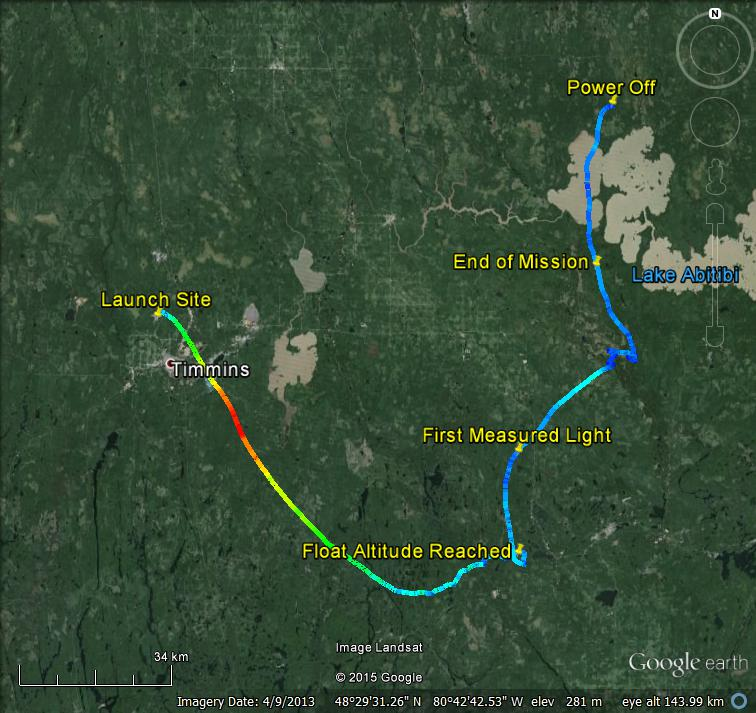
\includegraphics[width=1.0\textwidth]{./Images/5-1-AliGpsDataGoogleMaps.jpg}
    \caption[Flight Path of the Nimbus 7 Mission]{The GPS data from ALI during the Nimbus 7 mission generated via Google Earth. The colour of the line represents the absolute speed of the gondola during the mission. Important landmarks noted on the image. The end of mission represent the end of the primary aerosol mission. No GPS data was collected from ALI after the power down.}
    \label{fig:5.1:nimbus7FlightPath}
\end{figure}

\begin{figure}
    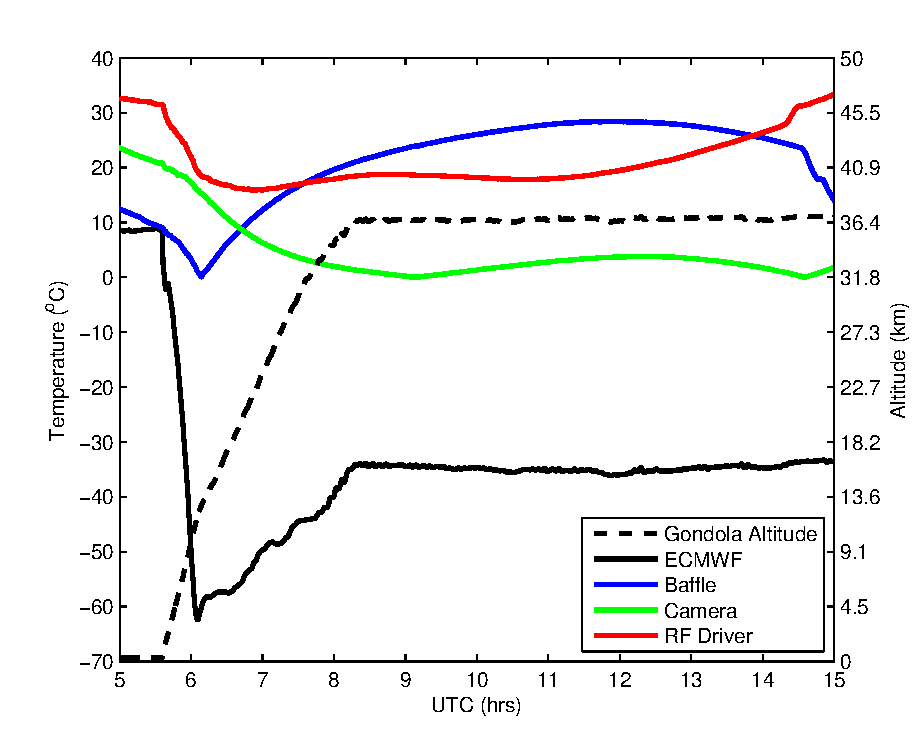
\includegraphics[width=1.0\textwidth]{./Images/5-1-FlightTemperatures.pdf}
    \caption[Flight Temperatures and Altitude Profiles from Nimbus 7]{Temperature and altitude profiles from the NIMBUS 7 flight.}
    \label{fig:5.1:nimbus7Temps}
\end{figure}

\begin{figure}
    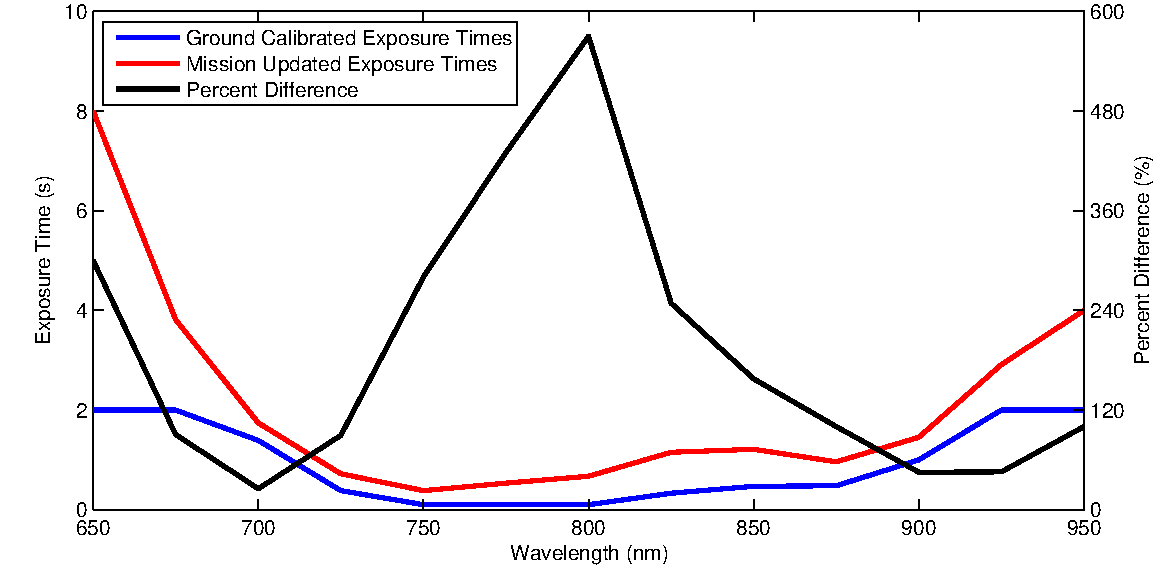
\includegraphics[width=1.0\textwidth]{./Images/5-1-ExposureTimeComparisons.pdf}
    \caption[Exposure Time Update During Balloon Flight]{During the flight the calibrated exposure time was updated as needed during the flight. The blue curve represents the exposure times from the ground calibration and the red curve is the recalibrate during the flight. The black curve is the percetn change in between the pre-flight calibrated results and the during flight calibration.}
    \label{fig:5.1:exposureTimeComparisons}
\end{figure}

After the completion of the mission, ALI was powered off at 17:15 UTC after successfully gathering 216 aerosol images. The gondola continued its flight until 21:54 UTC, a 16 hour 19 minute flight, at which point it landed approximately 70~km from Amos, Quebec or approximately 250~km from the launch facility . CARMEN-2 was recovered by the balloon recovery team and was return to base on September 21, 2015. It was removed from the gondola, repacked and travelled back to Saskatoon, Saskatchewan were processing of the data occurred. 
\section{Generation of Calibrated Radiances}
\label{sec:5.2:CalibratedRadiances}

ALI arrived back in Saskatoon on September XX, of 2015 and was unpacked and checked for any damages from either the transportation back to Saskatoon or from the landing at the end of the mission. No obvious damage had occurred to ALI and the instrument was functioning correctly. This allowed the complete data set record by ALI to be downloaded and used for aerosol profile processing. This section will undergo the method used to convert the raw data from the CCD to measured relative radiances used in the retrieval process.

The raw flight data, known as the level 0 data, must be converted to into level 1 relative radiances, which is the data normalized to a laboratory measurement value, before they can be used to retrieve aerosol extinction and particle size. The transformation includes removal of dark current, DC bias, stray light, and application of flat fielding calibration. Using the dark images from the assent of the flight combined with laboratory dark images a table of values based on exposure time and CCD temperature was computed to be able to remove the DC bias and dark current from each raw image accurately. Once completed, the time independent offset caused by the DC bias allows for the rest of the analysis to be preformed in counts per second, simplifying comparisons between images. %by taking the counts in the image and divided by the exposure time, in order to easily relate the radiance of different images directly to each other without having to scale the results with respect to the exposure time.

Stray light removal has always been difficult in atmospheric instrumentation due to the difficulty in accurately discerning the signal in regards to the stray light contamination. Furthermore, ALI's optical system has the further addition of unwanted light internal to the instrument because of the rejection of one of the polarizations due to the nature of the AOTF. The signal enters the optical system unpolarized, but only one polarization can have a consistent output angle from the AOTF. The entering light is passed through a linear polarizer with an extinction ratio of at least 100,000:1 to remove the unwanted polarization however a small percentage is not absorbed. Furthermore, a second linear polarizer is used after the AOTF to reject all of the unwanted radiance that did not meet the Bragg criteria and once again a small percentage of this radiance is not absorbed. The active filtering of the AOTF allows for an image to be measured when the filtering device is disabled, which is with no applied RF, allowing only the stray light to be captured by the measurement known as a `dark image', and during ALI's aerosol mode a `dark image' was captured before every measurement image. By removing the `dark images' from the signal-stray light contaminated images the end result is images that only contain the measured signal. The previous method was tested in the lab with a known source with even illumination across the field of view of the system, the resulting final image is left with a even decrease in intensity radiating from the center of the field of view as its expected with the known vignetting of ALI. The vignetting is caused by the aperture of the AOTF itself, by using a simple optical layout as chosen for the prototype the larger the angle for the field of view the more light that get blocked by the AOTF's apperture causing a known vignetting for the images and will need to be calibrated out of any measurements.

To finalize the data into level 1 relative radiances a flat fielding calibration is preformed, which involves taking all the incoming fielding of views and normalize them to be unity. The flat fielding coefficients needed to be applied not only spatially across each image but spectrally across a series of images. To determine the flat fielding coefficients ALI was set up in the lab viewing the light emitted from a 250~W quartz-tungsten halogen bulb that is passed through a diffusing plate to give an evenly distributed signal across the entire field of view of ALI. Measurements were taken at varying integration times at every wavelengths used in ALI's aerosol mode. Since ALI is most sensitive at 750~nm, it was chosen to be the reference point. The center pixels of the 750~nm images were used since they experience little vignetting, specifically the center 25 by 25 pixels. All pixels for every image were normalized to the mean of the reference point pixels. From these normalized images, the flat fielding coefficients were the values needed to multiply the normalized images to achieve unity. The coefficients were then averaged for each wavelength and applied to the flight data to yield the final relative radiances. In \autoref{fig:BeforeAfterImages} image number 212, a 750~nm image, is shown with a before and after comparison. The before image is the raw data directly after the mission with no calibrations preformed and the after image in the bottom panel is the same image after the all the calibrations have been applied.

%and used to normalized the full field of view across the whole spectrum to the center of the 750~nm images, thus giving a relative calibration of radiance referenced to this point. The process used to determine the flat fielding coefficients started with similar process used to remove the stray light during the mission post processing. The images had the DC bias and dark current removed for proper unbiased comparisons and converted to counts per second. Each value of every pixel in the active region of the CCD was normalized to the mean of the value on the center 25 by 25 pixels at 750~nm over all exposure times and trials. The coefficients for flat fielding can be determined as the values to yield a unified radiances of one across all field of views and wavelengths. These coefficients are then applied to the data from the flight that give relative radiances for each pixel.

To increase the precision of the measurements from the flight the images were averaged in cells of 25 horizontal pixels and vertical pixel averaging that would result in the measured radiances being on a 1~km vertical grid. Furthermore, a loss of resolution was speculated to occur in the flight data because of the drastic change in temperature of the optics during the flight which is a secondary reason for the pixel averaging. ALI radiance profiles from the complete mission from the 0\si{\degree} line of sight can be seen in \autoref{fig:AliRadiancesVectors} which includes wavelengths from 675-950~nm and generally have good internal agreement from 13 to 30~km. Images 207, 211, and 215 were selected to demonstrate subtle radiance differences between different horizontal lines of sights with each profile's respective error and can be seen in \autoref{fig:AliRadiances}. Lastly, images 204 to 216 were used to show the spectrum of relative radiances at a series of altitudes which is seen in \autoref{fig:AliSpectralRadiances}.

\begin{figure}
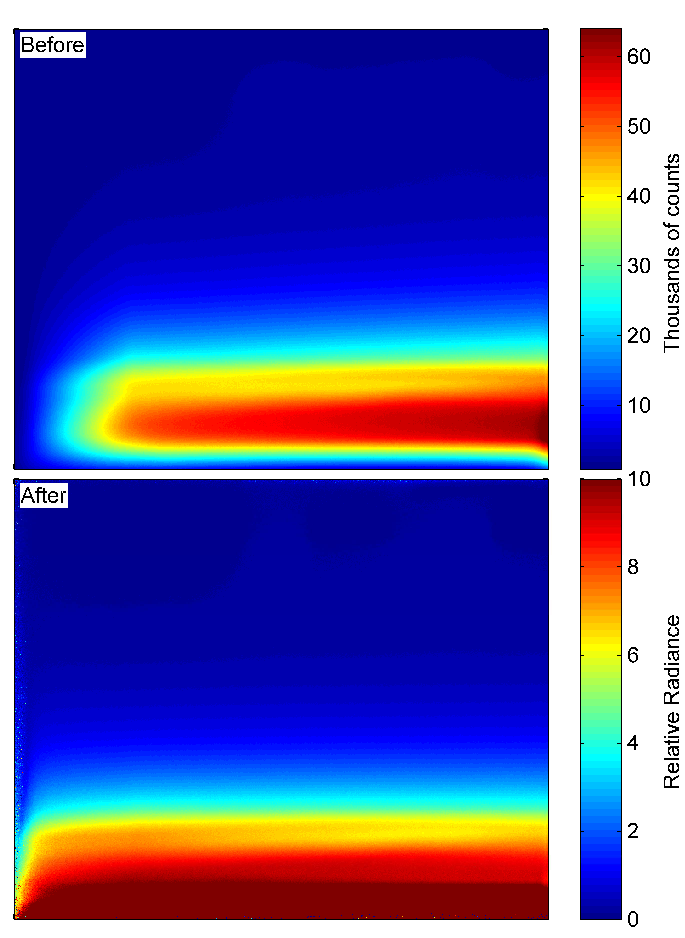
\includegraphics[width=1.0\textwidth]{./Images/5-2-BeforeAfterImage.pdf}
    \caption[TODO:Write This]{Comparison of the same image, image number 212, at 750~nm. The upper panel is the raw level 0 data and the lower panel is the relative radiance level 1 data.}
    \label{fig:5.2:BeforeAfterImages}
\end{figure}

\begin{figure}
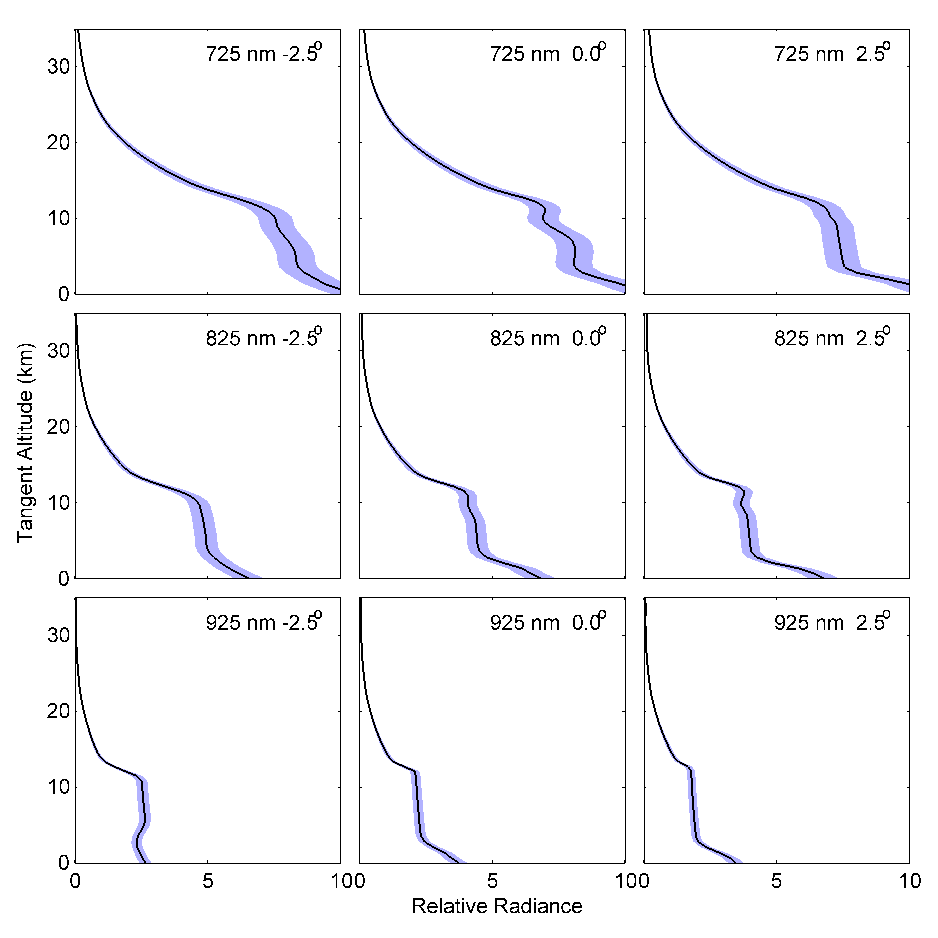
\includegraphics[width=1.0\textwidth]{./Images/5-2-AliRadiances.pdf}
    \caption[TODO:Write This]{Level 1 relative radiances as measured form ALI at approximately 14:20 UTC (images number 207, 211,and 215) looking 90\si{\degree} from the sun facing southwards. The top middle, and bottom row are measurements taken at 725, 825, and 925~nm respectively. The center column is viewing the atmosphere directly in front of ALI, While the left column is looking to the left at -2.5\si{\degree} and the right at 2.5\si{\degree}. }
    \label{fig:5.2:AliRadiances}
\end{figure}

\begin{figure}
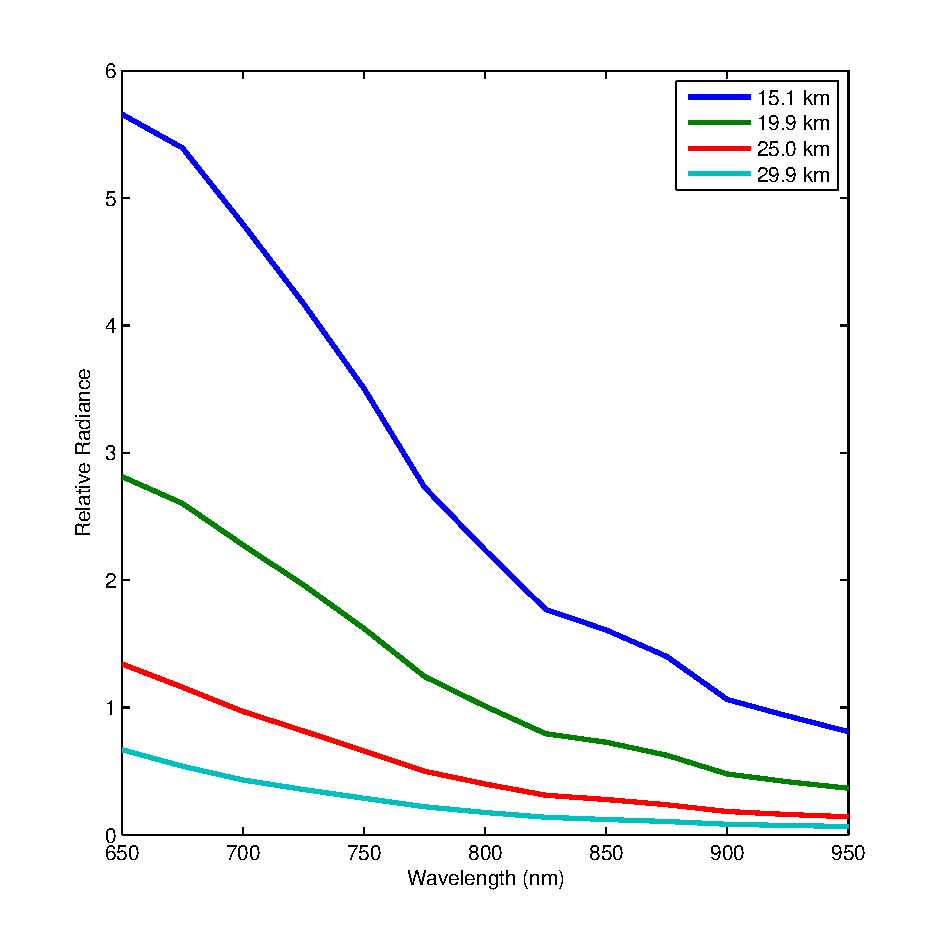
\includegraphics[width=1.0\textwidth]{./Images/5-2-AliSpectralRadiances.pdf}
    \caption[TODO:Write This]{Level 1 relative radiances spectrally from 650~nm to 950~nm as measured form ALI at approximately 14:20 UTC consisting of images number 204 to 216 looking 90\si{\degree} from the sun facing southwards. These spectral profiles are presented at several tangent altitudes with a horizontal field of view of 0\si{\degree}.}
    \label{fig:5.2:AliSpectralRadiances}
\end{figure} 
\section{Aerosol Retrievals}

Aerosol Retrival Info Goes Here

From paper

The modeled radiances were computed with the SASKTRAN radiative transfer engine \citep{Bourassa2008a} for for High Resolution (SASKTRAN-HR) \citep{Zawada2015} measurements using the newly developed polarization module \citep{Dueck2015}. The model uses a given atmospheric state to solve the radiative transfer equation to determine the final radiance at the observer that follows
\begin{equation}
    I(s_{1}) = I(s_{0})e^{-\tau(s_{0}, s_{1})}+\int^{s_{1}}_{s_{0}}k(s)J(s)e^{-\tau(s, s_{1})}ds
\end{equation}
where $I(s_{1})$ is the radiance at the observer through a path from $s_{0}$ to $s_{1}$, the first term is the contribution of light that is attenuated along the line of sight from the sun to the observer at $s_{1}$. The second term takes the source term, $J(s)$, which is the radiance scattered into the line of sight and integrates the path along line of sight with attenuation to determine the scattering contribution to the final radiance. The extinction, given by $k(s)$, is the sum of the number density, $n(s)$, multiplied by the scattering cross section, $\sigma(s)$, over all species and $\tau$ is the optical depth. The polarized output of SASKTRAN-HR gives the Stokes vectors for the radiance on its internal coordinate grid which can be retrieved from the model and then rotated to match ALI's coordinate system.

The relative radiance level 1 data from ALI are used create a measurement vectors, $y$, in the following form
\begin{equation}
    \mathbf{y} = \log\left(\frac{\mathbf{I}(\mathbf{z},\lambda)}{I(z_{ref},\lambda)}\right)-\log\left(\frac{\mathbf{I}_{rayleigh}(\mathbf{z},\lambda)}{I_{rayleigh}(z_{ref},\lambda)}\right)
    \label{eqn:measurementVector}
\end{equation}
where $\mathbf{I}(\mathbf{z},\lambda)$ is the measured radiance from ALI and $I(z_{ref},\lambda)$ is the radiance at a reference altitude used to normalize the signal from a high altitude where there is little aerosol contribution, for ALI the highest possible altitude where the signal is above the noise threshold is around 25-30~km tangent height. The second term is modeled values from SASKTRAN-HR with only background neutral atmosphere to remove the rayleigh signal from the measured radiances which is done to improve the speed of the convergence of the retrieval. The ALI measurement vector is similar to the measurement vector used for the OSIRIS retrieval \citep{Bourassa2007,Bourassa2011}. A base aerosol state or a priori, $\mathbf{x}$, for aerosol extinction profile is used in the SASKTRAN-HR model. The forward model vector is constructed similarity to the measurement vector and follows.
\begin{equation}
    \mathbf{F}(\mathbf{x}) = \log\left(\frac{\mathbf{I}_{mod}(\mathbf{z},\lambda)}{I_{mod}(z_{ref},\lambda)}\right)-\log\left(\frac{\mathbf{I}_{rayleigh}(\mathbf{z},\lambda)}{I_{rayleigh}(z_{ref},\lambda)}\right)
    \label{eqn:forwardModel}
\end{equation}
where $I_{mod}(z,\lambda)$ is the modeled radiance for the measurement and $I_{mod}(z_{ref},\lambda)$ is the measurement at the same reference altitude for normalization. The forward model is used in combination with the measurement vector to update the extinction profile in the Multiplicative Algebraic Reconstruction Technique (MART) algorithm which was developed for use in the OSIRIS retrievals \citep{Bourassa2012a} with the following iterative technique
\begin{equation}
    x_{i+1} = x_{i}\sum_{j}\frac{y_{j}}{F(z_{j})}W_{ij}
\end{equation}
where $x_{i}$ is the aerosol extinction at each shell altitude, $i$ and $j$ is the tangent point from the measurements. $W_{ij}$ is the weighting matrix that relates the importance of each measurement vector to each shell altitude. This method was outlined by \cite{Degenstein2009} and allows for fast retrievals without calculating a Jacobian.

An error estimation was also needed to be able to fully classify the capabilities of ALI and was performed using a perturbation method. Once a retrieval has been completed for an image the result is used to estimate the error in the returned extinction. For each altitude, the measurement vector is perturbed by the error resulting form the level 0 to level 1 data conversion parameters used and from the readout electronics. The MART retrieval is rerun and the change of the extinction is determined. These are compiled to form a gain matrix, $\mathbf{G}$, with size is $n$ by $m$ which are the shell altitudes and the tangent altitudes grids respectively, with elements $g_{ij}$. The error at each retired altitude is then given by
\begin{equation}
    e_{i} = \left(\sum_{j}g_{ij}g_{ji}\right)^{0.5}
\end{equation}
which gives the error at at retrieved altitude.

Results:

In order to be able to use the ALI data in the MART method certain quantities were needed for the model; albedo, ozone concentration and cross sections, and aerosol cross sections. The albedo is required since an absolute radiance calibration was never preformed with ALI and the albedo cannot be determined directly form ALI's measurements, which is important since the amount of ground scatter in SASKTRAN-HR must correspond to the ground scatter during ALI's flight. Second, the ozone absorbtion features from the Chappuis band appear in the ALI measurements from 650 to 750~nm. The absorbtion must be accounted for to not artificially change the determined aerosol profiles. The ozone profiles were acquired from OSIRIS. Five scans that were within 48 hours of the balloon flight and  within 500~km of the launch facility were averaged together to be the ozone profile used in the SASKTRAN-HR model, with cross sections from \cite{Burrows1999}. The albedo is from the ADAM database which has monthly values for albedo over the surface on earth at a resolution of 0.1\si{\degree}~x~0.1\si{\degree} grid at 1~nm spectral resolution \citep{Muller2013}. The aerosol cross sections come from the Mie scattering derivation that was originally proposed by Mie and was implemented efficiently by \cite{Wiscombe1980}. For the purpose of the retrieval an a priori was used with a mode radius of 0.08~$\si{\micro\metre}$  and a mode width of 1.6 which is considered a standard size distribution for aerosol \citep{Deshler2003}.

The complete mission consisted of 216 images that were recorded in illuminated conditions. The MART retrieval method was run on a select signal set for the purpose of the analysis, specifically the last complete set of images from 650 to 950~nm consisting of images 204-216. They were chosen due to being the last in the mission and the sun was the highest in the sky giving the brightest atmosphere leading to the best signal to noise during the mission. A sample of the retrieval set can be observed in \autoref{fig:AliRetreivals} which highlights the 725, 825, and 925~nm retrievals. The left panels shows the measurement vector from ALI in black with the forward model radiance profile from SASKTRAN-HR in blue. For each of the wavelengths, the algorithm determines altitudes where the value of the measurement vector is less than the known noise and does not allow aerosol to be retrieved in those regions. Instead the scaling factor, given by $\alpha = yF^{-1}$ is scaled to the aerosol profile above and below the last retrieved point to keep the aerosol profile smooth, as discontinuities are nonphysical and can lead to a convergence failure in the MART algorithm. The middle panel shows the convergence between the measurement vector and the forward model result. For the center wavelengths, being 700-875~nm, a difference of less than 2\% is seen from 12 to 22~km with a few outliers.

The aerosol profile for the three wavelengths is shown in blue with the shading representing the error for the retrieval strictly based on measurement error and neglecting any model and atmospheric state errors. The green curve is the average 750~nm aerosol extinction profiles of the same five OSIRIS scans used for the ozone profile and red is the 750~nm aerosol extinction from SALOMON \citep{Berthet2002} which was launched from the Timmins balloon base as the Nimbus 5 mission on September 12, 2014. The aerosol extinction for ALI and OSIRIS are within 50\% of each other for a majority of the 725~nm and 825~nm profile while the upper altitude of the 925~nm are considerable different, in some places over 100\% difference occurs. However, agreement is best for 750~nm profile and displays a reasonable spectral dependance to also should be noted that the three instruments follow the same overall shape.  First, a bend in the profile occurs at approximately 25~km, then increases approximately linearly until 15~km where aerosol extinction leaves the linear trend and forms the peak of the measurement. The agreement in shape is an excellent result for the ALI mission due to the good numerical comparison with OSIRIS as well as the overall profile shape agreement between all three instruments.

\begin{figure}
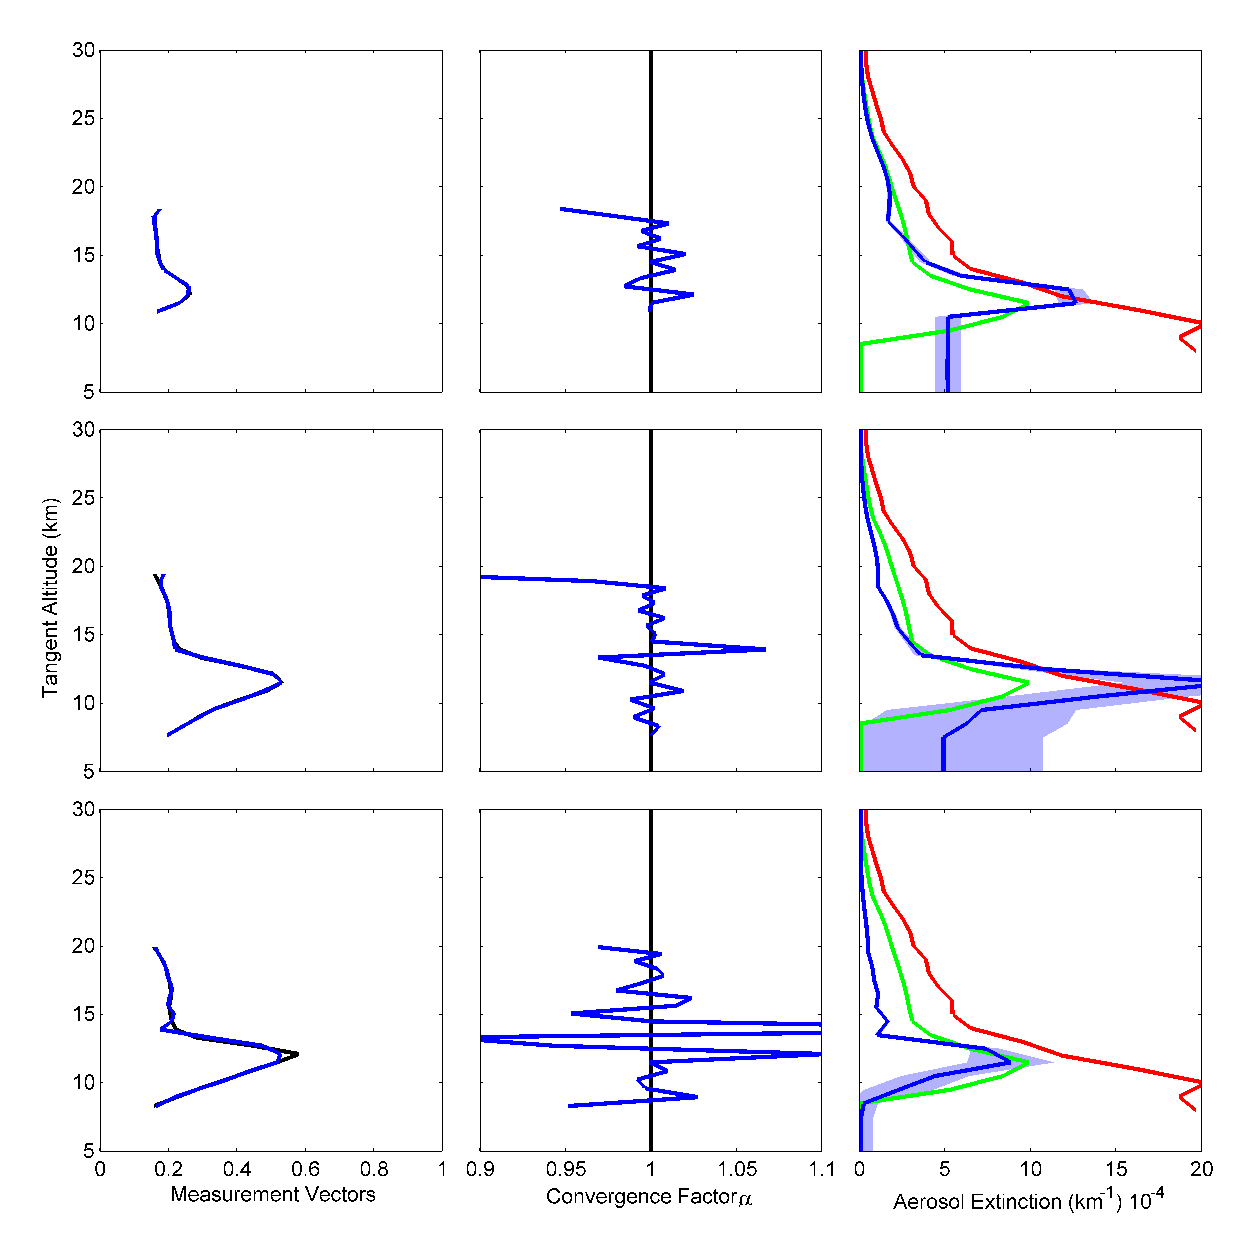
\includegraphics[width=1.0\textwidth]{./Images/5-3-AliRetreivals.pdf}
    \caption[TODO:Write This]{An example of three aerosol retrievals from images 207, 211, and 215, with center wavelengths of 725, 825, and 925~nm respectively and vertically displayed in the figure from top to bottom. The left column shows the measurement vector, $y$, in black with the retrieved forward model, $F$, in blue. The center column shows the ratio of the $y$ over $F$ known as $\alpha$ and is the convergence factor between the ALI measurement and the forward model. The final column is ALI aerosol extinction in blue with the associated error represented by the light blue shading. The green is 750~nm aerosol extinction measured by OSIRIS, and red is 750~nm extinction as measures by SALOMON.}
    \label{fig:5.3:AliRetreivals}
\end{figure} 
\section{Particle Size Determination}
\label{sec:5.4:ParticleSizeDetermineation}

With assumed particle size distributions for the retrievals aerosol extinction form the previous section there is a unfavour wavelength dependance on the values of the extinction. In this section a discussion of the requirement to achieve full particle size information will be underwent followed by the method used to determine some particle size used on the ALI measurement s and the results with with updated extinction profiles.

\subsection{Particle Size Sensitivity}

To rectify the problem with the dependance between the extinction and wavelength a method will be preformed on the data in order to try to extract some particle size information But first a look into the information of particle size from limb measurements must be explored. From work done by \citep{Rieger2014} shows that different particle size distributions can effect the aerosol measurement vector. He uses an OSIRIS scan geometry and calculates the respective measurement vectors for a series of particle sizes which can be seen in reproduction of \autoref{fig:5.4:AerosolMeasurementParticleSizeInfo}. In panel A three different log-normal distributions are used which give a near identical measurement vector at 750~nm with simulation of the atmosphere with SASKTRAN. The three profiles are in blue is a single fine mode particle size distribution with a mode radius and width of 0.08~\si{\micro\meter} and 1.6 respectively, black is a bimodal particle size distribution the simulates volcanic conditions with the mode radius and width of 0.08~\si{\micro\meter} and 1.6 for the fine mode and 0.4~\si{\micro\meter} and 1.2 for the coarse mode, lastly red is a representative size distribution with mode radius and width of 77~\si{\micro\meter} and 1.75. Panel B shows the measurement vectors calculated with the three distributions across a series of wavelengths. The third panel, panel C, shows the difference of the measurement vectors compared to the bimodal distribution. Sensitivity to particle size is only seen past 800~nm measurement but great sensitivity does not occur until measurement recorded out to 1500~nm. Furthermore an error of 1\% in the radiance yields a relative error in the bimodal distribution measurement vector shown by the gray shading.

\begin{figure}
\centering
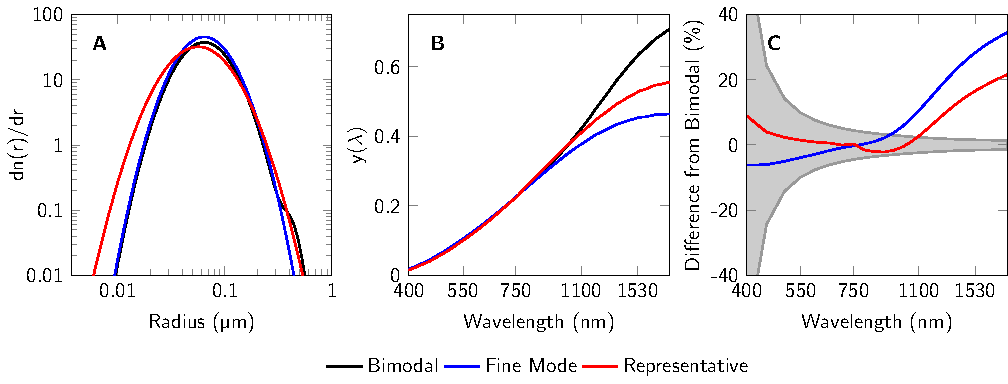
\includegraphics[width=1.0\textwidth]{./Images/5-4-AerosolMeasurementParticleSizeInfo.pdf}
    \caption[Aerosol Measurement Vectors Sensitivity to Particle Size]{Reproduced from \citep{Rieger2014}. For OSIRIS scan 6432001 aerosol measurement vectors were calculated at 22.5~km. (A) The three size distributions used in the study. (B) The measurement vectors calculated via the SASKTRAN simulation (C) The relative percent difference of the fine and representative distributions with respect to the bimodal distribution. A 1\% error is the radiance yields an uncertainty in the bimodal measurement vector shown by the grey shading.}
    \label{fig:5.4:AerosolMeasurementParticleSizeInfo}
\end{figure}

For ALI measurement were only gathered between 650 and 950~nm in wavelength, due to the CCD camera not having the required efficiency sample at wavelengths above this point. As such ALI only has some sensitivity to particle size form the longer wavelengths and only a small amount. As such it is not possible to determine both the mode radius and mode width due to information poor wavelengths. Instead the data from ALI will be used to determine the Angstr\"{o}m exponent. The Angstr\"{o}m exponent is an approximation to Mie scattering since the value of the Angstr\"{o}m exponent, $\alpha$, is an analogy to particle size. The scattering cross section for aerosol is dependant the particle size distribution assuming since the number density must be a constant across wavelength, as such the extinction value changes with a change in cross section. From \autoref{eqn:5.4:agstromCoefficient} the particle size profile from a series wavelength can be determined from the Angst\:{o}m exponent.Lower Angstr\"{o}m exponents correspond to larger particle sizes and vice versa for small particle sizes. Since the measurements observe relatively the same atmosphere over the time of one complete aerosol cycle; the differences between extinction ratios at the different wavelength can be used to gather a understanding of aerosol particle size in the form
\begin{equation}
    \frac{n\sigma}{n_{0}\sigma_{0}} = \left(\frac{\lambda}{\lambda_{0}}\right)^{-\alpha}
    \label{eqn:5.4:agstromCoefficient}
\end{equation}
where $n$ is the aerosol concentration, and $\sigma$ is the scattering cross section. For the 750~nm wavelength for a variety of mode radius and widths a change in the cross section can be observed in \autoref{fig:5.4:scatteringCrossSections}. The Angstr\"{o} exponent can also be determine  fitting a line through a series of points by rearangeing \autoref{eqn:5.4:agstromCoefficient} into the following
\begin{equation}
    \alpha = -\frac{\log(n\sigma)-\log(n_{o}\sigma_{o})}{\log(\lambda)-\log(\lambda_{o})}
    \label{eqn:5.4:agstromCoefficientSlope}
\end{equation}
which show the Anstr\"{o}m exponent in simple the slope of the log of the extinction over the log of the wavelengths.

\begin{figure}
\centering
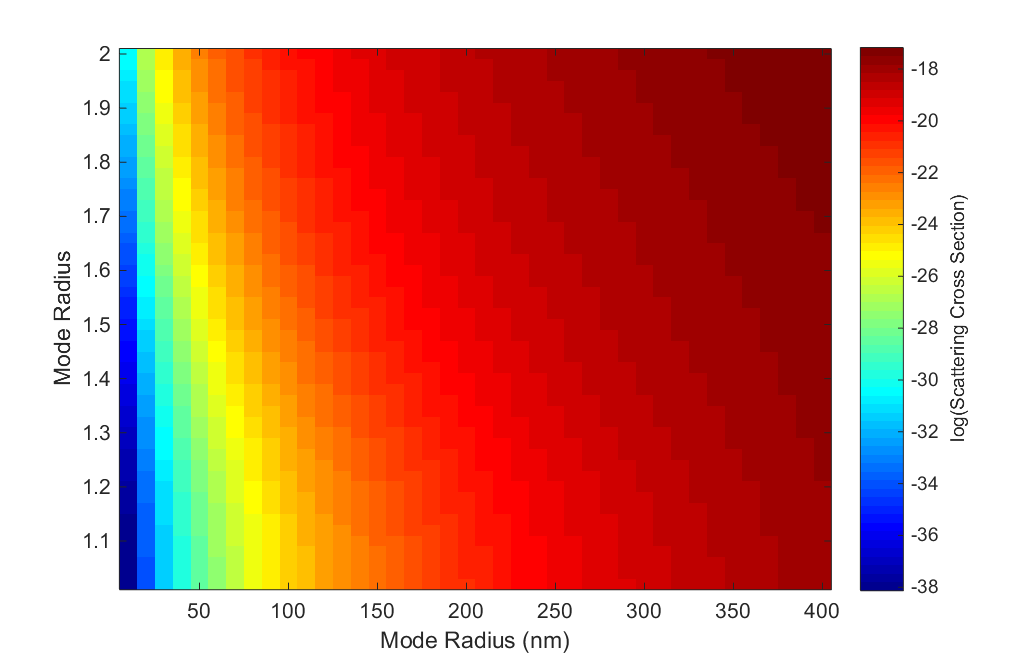
\includegraphics[width=1.0\textwidth]{./Images/5-4-CrossSectionDependance.pdf}
    \caption[Log of Scatting Cross Section for Various Mode Radii and Widths]{Computed with the optical properties of the SASKTRAN engine. This varation of the corss section with respect to the mode radius and width allows for some determination of the particle size distribution through the Angstr\:{o} exponent.}
    \label{fig:5.4:scatteringCrossSections}
\end{figure}

\subsection{Particle Size Retrieval Method and Results}

Once the retrieval has been preformed for a complete series of wavelengths; determination of the Angstr\"{o}m exponent occurs which is preformed in a similar manor as outlined by \cite{Rault2013} for the OMPS aerosol particle size retrieval.  For the retrieval described here a single mode log-normal distribution is assumed with a mode radius, $r_{g}$, and the mode width, $\sigma_{g}$, which is the same as the OSIRIS version 5.07 aerosol product of 0.08\si{\micro\meter} and 1.6 respectively. The process for the retrieval is as follows:
\begin{enumerate}
    \item Set up a MART retrievals for all wavelengths measured by ALI was a mode radius and width of 0.08\si{\micro\meter} and 1.6 respectively.
    \item Preform the MART retrieval for each wavelength.
    \item For all wavelengths determine the maximum minimum retrial altitude and minimum maximum retrieval altitude. These will be the bound for for the particle size retrievals.
    \item For each valid tangent height fit a least squares line through the extinctions and wavelengths via \autoref{eqn:5.4:agstromCoefficientSlope} to determine the Angstr\"{o}m exponent. A wavelength at a altitude was rejected if the forward model at that shell altitude was not within 3\% of the measurement vector.
    \item For each tangent height convert the Angstr\"{o}m exponent into a mode radius assuming a mode width of 1.6.
    \item Take the median of all the determined mode radii and use this as the new values for the mode radius. If this value is the same as the previous iteration stop the retrieval as the solution has converged, If it is different change the mode radius in the model to the new mode radius and repeat the sequence from step 2.
\end{enumerate}
This method generally achieved convergence within 4-5 iterations.

A sample particle size retrieval is shown in \autoref{fig:5.4:ParticleSize} for the cycle consisting of images 204-216. The first panel of \autoref{fig:ParticleSize} shows the median Angstr\"{o}m exponent that was determined after each iteration and convergence can be seen after a couple iterations. The initial guess for the mode radius was changed to several different values and each run of the model resulted in the same final retrieved mode radius. The particle size determined for ALI in the last complete set of aerosol images can be seen in the second panel of \autoref{fig:ParticleSize} which yields a final Angstr\"{o}m exponent of between 2 and 3 throughout the altitude range from 13 to 22~km. Assuming a mode width of 1.6 yields a median mode radius of 0.105~\si{\micro\metre}. The final panel shows the least squares for the 20.5~km tangent altitude for this case only 11 of the 13 possible wavelengths contributed to the determination of the Angstr\"{o}m exponent.

\begin{figure}
\centering
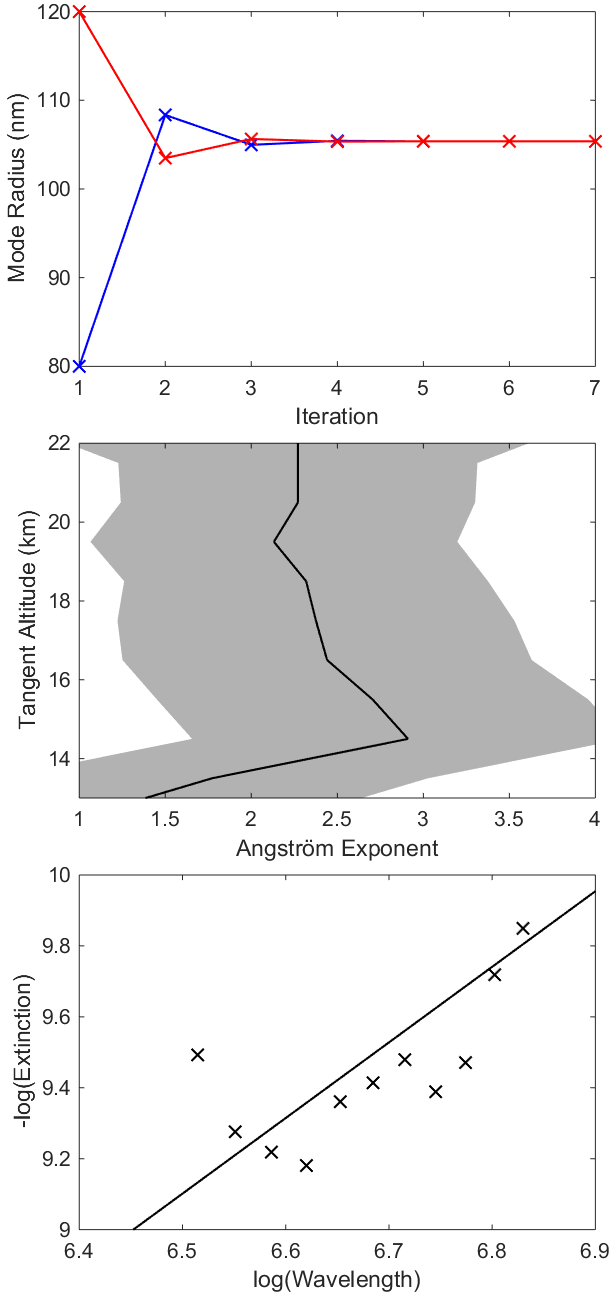
\includegraphics[width=0.5\textwidth]{./Images/5-4-ParticalSize.pdf}
    \caption[Particle Size Retrieval]{The top panel shows the convergence of two sample particle size retrievals over the iterations, blue and red represent a priori of 0.08 and 0.12~\si{\micro\metre} respectively. Both initial state converge to the same value over approximately 4 iteration in the particle size retrieval method. The second panel is the final Angstr\"{o}m exponents determined for images 204-217 during the Timmins 2014 campaign and are in black as the final profile was almost identical after each particle size retrieval, the shading represents the error associated with the least squares fit. The last panel demonstrate a least squares fit to determine the Angstr\"{o}m exponent at 20.5~km shell altitude.}
    \label{fig:5.4:ParticleSize}
\end{figure}

The error in the Angstr\"{o} exponent was determined looking at the error in the slope possible from the least squares method. Assuming no error in the extinction points the error in the slope is given by
\begin{equation}
    \delta\alpha = \frac{s}{SS_{xx}}
\end{equation}
where $s$ is
\begin{equation}
    s = \sqrt{\frac{SS_{yy}-\alpha SS_{xy}}{n-2}},
\end{equation}
and $SS_{xx}$, $SS_{yy}$, and $SS_{xy}$  are the sum of squares of the wavelength, aerosol extinction, and cross term between the wavelength and aerosol extinction and $n$ is the number of points. However there is and associated error with each aerosol extinction profile. To determine the error on the Angstr\"{o}m exponent accounting for the precision in the aerosol extinction the error on the slope was calculated 10,000,000 times with each iteration a random amount of error from he known range was added to each extinction point. Then the mean from the all the errors of the least squares fit was used as the fine precision estimate on the Angstr\"{o}m coefficient which can be seen in the second panel of \autoref{fig:5.4:ParticleSize}.

The extinction cycle similar to \autoref{fig:5.3:AliAerosolCycleNoPartSize} is shown in \autoref{fig:5.4:AliAerosolCycle} except with updated particle size parameters form the retrieval. the aerosol extinction profiles now shows the characteristic decrease in aerosol extinction that is expected as wavelength increase. this extinction is self consistent with Mie theory and give some validity to the retrieved particle sizes determined from ALI.

\begin{figure}
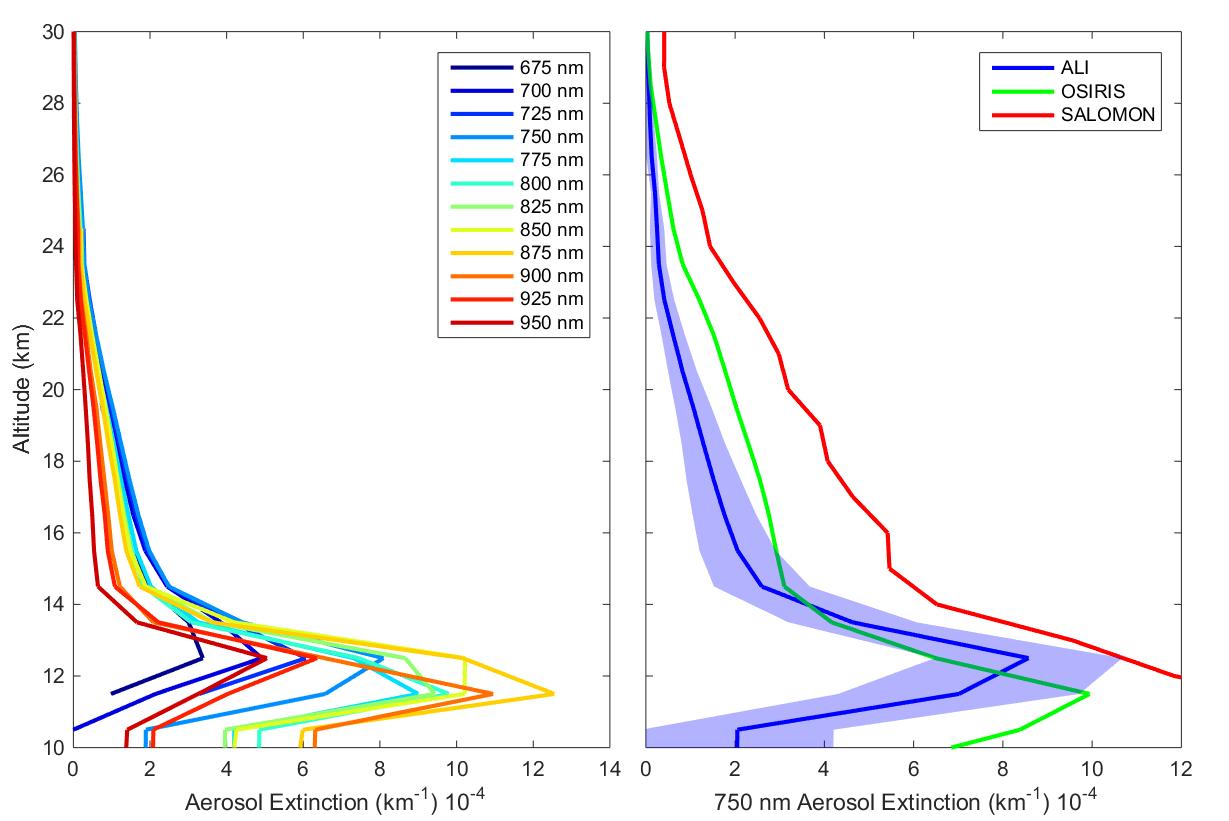
\includegraphics[width=1.0\textwidth]{./Images/5-4-FullAerosolCycleComparison.pdf}
    \caption[Aerosol Retrievals with Corrected Particle Size for All Wavelengths and 750~nm Comparison with OSIRIS and SALOMON]{Left is the retrieved aerosol extinction profiles from the last complete cycle consisting of images 205 to 216 from the 0.0\si{\degree} horizontal line of sight. Right is the 750~nm ALI aerosol extinction in blue with its error represented by the shading compared to the 750~nm extinction measured by OSIRIS and SALOMON in green and red respectively.}
    \label{fig:5.4:AliAerosolCycle}
\end{figure}   
\section{Comparisons and Validation}

Comparisons and Validations Info

\subsection{SOLAMON}
\subsection{OSIRIS}
\subsection{OMPS} 
\input{./Chapter6/FutureWorkandConclusions.tex}

\uofsbibliography[thesis]{BiBTex}

\uofsappendix

\chapter{ALI Hardware Components}

Add separate tex file for this later.

\chapter{ALI Software Commands}

Add separate tex file for this later

\end{document} 